\chapter{Linear Algebra and Geometry I}

\newpage

\section{Linjära ekvationssystem}

\textbf{3 gundläggande operationer för att lösa linjära ekvationer}
\begin{align*}
  &\quad (1) \text{ (Tvåpilar) Byt om på två ekvationer} \\
  &\quad (2) \text{ (Labbda) Multiplicera båda sidorna av en ekvation med } \lambda \neq 0 \\
  &\quad (3) \text{ (Labda pil) addera } \lambda
  \text{ gånga en ekvation till en annan ekvation} \\  
\end{align*}


\textbf{Generall lösning}
\begin{align*}
  &\quad  \left\{\begin{array}{l}
  a_{1} x+b_{1} y=c_{1} \\
  a_{2} x+b_{2} y=c_{2}
  \end{array}\right. \\
  &\quad  \text{Lambda pil upp}\left\{\begin{array}{l}
  a_{1} x+b_{1} y=c_{1} \\
  a_{2} x+b_{2} y=c_{2}
  \end{array}\right. \\
  &\quad  \text{Ger nya ekvationssystemet} \\
  &\quad  \text{Lambda pil upp}\left\{\begin{array}{l}
  (a_{1}+\lambda a_{2})x + (b_{1}+\lambda b_{2})y=c_{1} + \lambda c_{2} \\
  a_{2} x+b_{2} y=c_{2}
  \end{array}\right. \\
  &\quad  \text{-Lambda pil upp}\left\{\begin{array}{l}
  (a_{1}+\lambda a_{2})x + (b_{1}+\lambda b_{2})y=c_{1} + \lambda c_{2} \\
  a_{2} x+b_{2} y=c_{2}
  \end{array}\right. \\
  &\quad
\end{align*}

\textbf{Exempel linjär ekvationssystem}
\begin{align*}
  &\quad  \left\{\begin{array}{l}
  2x+3y=4 \\
  3x-y=6
  \end{array}\right. \\
  &\quad \\
  &\quad  \text{Andvänder rad operationer för att lösa ekv systemet} \\
  &\quad  (-\frac{3}{2})\text{pil ned}\left\{\begin{array}{l}
  2x+3y=4 \\
  3x-y=6
  \end{array}\right. \\
  &\quad
  (3x-y) -\frac{3}{2} (2x+3y)=6 -\frac{3}{2} \cdot 4 \Leftrightarrow{} \\
  &\quad
  (3-\frac{3}{2}\cdot 2) x + (-1 -\frac{9}{2}) y = 6 -6
  \Leftrightarrow-\frac{11}{2}y = 0 \\
  &\quad  (-\frac{2}{11})\text{ned}\left\{\begin{array}{l}
  2x+3y=4 \\
  -\frac{11}{2}y = 0
  \end{array}\right. \\
  &\quad  (-3)\text{pil upp}\left\{\begin{array}{l}
  2x+3y=4 \\
  y=0
  \end{array}\right. \\
  &\quad  (\frac{1}{2})\text{upp}\left\{\begin{array}{l}
  2x=4 \\
  y=0
  \end{array}\right. \\
  &\quad  \left\{\begin{array}{l}
  x=2 \\
  y=0
  \end{array}\right. \\
  &\quad \\
  &\quad  \text{\textbf{Kontrol:} stoppar in $x$ och $y$ i ekvationerna} \\
  &\quad  2\cdot{2}+3\cdot{0}=4 \text{ (stämmer)} \\
  &\quad  3\cdot{2}-\cdot{0}=6 \text{ (stämmer)} \\
\end{align*}


\newpage

\subsection{Total Matris}
\textbf{Termonologi}
\begin{itemize}
\item Rader och Kolonner: Rader är vågräta delen av matrisen (ekvationen)
  Kolonner är lodräta delen (koificenterna)
\item ledande ekvivalent: 
\item trappstegs matris: När ledande ekvivalent är i trapp form går ned max ett steg
\item rad kanonisk: När alla av de ledande ekvivalent inte har någon i samma kolonn
\end{itemize}

  
\textbf{Exempel matriser}
\begin{align*}
  &\quad \left\{\begin{array}{rr}
  x+2 y+ & z=-1 \\
  2 x+(a+3) y+ & 3 z=-4 \\
  x+(3-a) y+(a-2) z & =a-1
  \end{array}\right. \\
  &\quad \left(\begin{array}{ccc|c}
    1 & 2 & 1 & -1 \\
    2 & a+3 & 3 & -4 \\
    1 & 3-a & a-2 & a-1
  \end{array}\right) \\
  &\quad (-1 \text{ rad1 till rad2}), (-2 \text{ rad1 till rad3}) \\
  &\quad \left(\begin{array}{ccc|c}
    1 & 2 & 1 & -1 \\
    2 & a-1 & 1 & -2 \\
    0 & 1-a & a-3 & a
  \end{array}\right) \\
  &\quad \left(\begin{array}{ccc|c}
    1 & 2 & 1 & -1 \\
    0 & a-1 & 1 & -2 \\
    0 & 0 & a-2 & a-2
  \end{array}\right) \\
  &\quad a \neq 1 \land a \neq 2 \\
  &\quad (\frac{1}{a-2} \text{rad 3}) \\
  &\quad \left(\begin{array}{ccc|c}
    1 & 2 & 1 & -1 \\
    0 & a-1 & 1 & -2 \\
    0 & 0 & 1 & 1
  \end{array}\right) \\
  &\quad (-1 \text{rad 3 till rad 2}), (-1 \text{rad 3 till rad 1}) \\
  &\quad \left(\begin{array}{ccc|c}
    1 & 2 & 0 & -2 \\
    0 & a-1 & 0 & -3 \\
    0 & 0 & 1 & 1
  \end{array}\right) \\
  &\quad (\frac{1}{a-1} \text{rad 2}) \\
  &\quad \left(\begin{array}{ccc|c}
    1 & 2 & 0 & -2 \\
    0 & a-1 & 0 & -3 \\
    0 & 0 & 1 & 1
  \end{array}\right) \\
  &\quad \left(\begin{array}{ccc|c}
    1 & 2 & 0 & -2 \\
    0 & 1 & 0 & \frac{3}{1-a} \\
    0 & 0 & 1 & 1
  \end{array}\right) \\  
  &\quad (-2 \text{rad 2 till rad 3}) \\
  &\quad \left(\begin{array}{ccc|c}
    1 & 0 & 0 & -2 - \frac{6}{1-a} \\
    0 & 1 & 0 & \frac{3}{1-a} \\
    0 & 0 & 1 & 1
  \end{array}\right) \\  
  &\quad \left\{\begin{array}{rr}
  x & = -2 - \frac{6}{1-a} \\
  y & = \frac{3}{1-a} \\
  z & = 1
  \end{array}\right. \\
  &\quad \\
  &\quad \text{\textbf{Kontroll:} stoppar in x,y,z i ekvationerna} \\
  &\quad \left\{\begin{array}{r}
  \left(\frac{2 a-8}{1-a}\right)+\quad 2 \cdot\left(\frac{3}{1-a}\right)+\quad 1=-1 \\
  2 \cdot\left(\frac{2 a-8}{1-a}\right)+(a+3) \cdot\left(\frac{3}{1-a}\right)+\quad 3 \cdot 1=-4 \\
  \left(\frac{2 a-8}{1-a}\right)+(3-a) \cdot\left(\frac{3}{1-a}\right)+(a-2) \cdot 1=a-1
  \end{array}\right.
\end{align*}


\newpage

\section{Vektorer/koordinater i planet och rummet}
% geogebra: https://www.google.com/search?q=geogebra&source=lmns&bih=945&biw=1910&hl=en&sa=X&ved=2ahUKEwjmtZ-q9c7rAhUCxSoKHVRHCA8Q_AUoAHoECAEQAA
\textbf{Räkne regler vektorer}
\begin{align*}
  &\quad \text{A1 } \vec{u} + \vec{v} = \vec{v} + \vec{u} \\
  &\quad \text{A2 } \vec{u} + (\vec{v}+\vec{w}) = (\vec{v}+\vec{u}) + \vec{w} \\
  &\quad \text{A3 } \vec{u} + \vec{0} = \vec{u} \\
  &\quad \text{A4 } \vec{u} + \vec{v}  = \vec{0} \Leftrightarrow \vec{v} = \vec{-u} \\
  &\quad \text{M1 } 1\vec{u} = \vec{u} \\
  &\quad \text{M2 } k(l\vec{u}) = (kl)\vec{u} \\
  &\quad \text{M3 } (k+l)\vec{u} = k\vec{u} + l\vec{u} \\
  &\quad \text{M4 } k(\vec{u}+\vec{v}) = k\vec{u} + k\vec{v} \\
\end{align*}

\begin{align*}
  &\quad \vec{a} = \begin{pmatrix}
  a_1 \\
  a_2 
  \end{pmatrix} \text{ för } \mathbb{R}^2 \\
  &\quad \\
  &\quad \vec{a} = \begin{pmatrix}
  a_1 \\
  a_2 \\
  a_3
  \end{pmatrix} \text{ för } \mathbb{R}^3 \\
\end{align*}

\textbf{Definition: Parallela vektorer}
\begin{align*}
  &\quad \text{Parallela omm } \exists{k}: \vec{u} = k\vec{v} \lor k\vec{u} = \vec{v}
\end{align*}


\subsection{Bas}
Standard bas är välbikant då i planet är x och y axeln medans i ett rum är x, y och z.
Baser som inte är standard är vektorer som ej är parralella som då skappar axlar som ej
behöver vra vinkelräta. \newline

\textbf{Definition: Bas}
\begin{align*}
  &\quad  \text{Bas i plan } \forall{\vec{x}},\exists{k_1,k_2}:
  \vec{x} = k_1\vec{u} \lor k_2\vec{v} \\
  &\quad  \text{Bas generell } \vec{x} = k_1\vec{u_1}+k_2\vec{u_2}+ \ldots +k_n\vec{u_n} \\
  &\quad \underline{u}=(\vec{u_1}\vec{u_2}\ldots\vec{u_n}) \\
  &\quad
  \vec{e_1}=\begin{pmatrix}  1 \\  0 \\  0  \end{pmatrix}
  \vec{e_2}=\begin{pmatrix}  0 \\  1 \\  0  \end{pmatrix}
  \vec{e_3}=\begin{pmatrix}  0 \\  0 \\  1  \end{pmatrix} \\
\end{align*}

\textbf{Exempel: kordenatar för vektor i bas}
\begin{align*}
  &\quad \text{Låt: }
  \vec{u}=\begin{pmatrix}  2 \\  1   \end{pmatrix},
  \vec{v}=\begin{pmatrix}  -2 \\  1   \end{pmatrix} \\
  &\quad  \text{Hitta kordenarterna för vektorn }
  \vec{x}=\begin{pmatrix}  0 \\  6   \end{pmatrix} \\
  &\quad \\
  &\quad  \text{Lösning: vi måste hittar realla tal $k_1$ och $k_2$ så att } \\
  &\quad
  \begin{pmatrix}  0 \\  6   \end{pmatrix} =
  k_1\begin{pmatrix}  2 \\  1   \end{pmatrix} 
  +k_2\begin{pmatrix}  -2 \\  1   \end{pmatrix} =
  \begin{pmatrix}  2k_1-2k_2 \\  k_1+k_2   \end{pmatrix} \\
  &\quad 
  \left\{\begin{array}{r}
  2k_1-2k_2 = 0 \\
  k_1+k_2 = 6 
  \end{array}\right. \Rightarrow{}
  \begin{pmatrix}  k_1 \\  k_2   \end{pmatrix} =  \begin{pmatrix}  3 \\  3   \end{pmatrix} \\
\end{align*}


\textbf{Exempel: Om det är en bas}
\begin{align*}
  &\quad \text{För vilken värde på a är vektorerna en bas för } \mathbb{R}^3 \\
  &\quad
  \vec{u_1} = \begin{pmatrix}  1 \\  2 \\  3  \end{pmatrix},
  \vec{u_2} = \begin{pmatrix}  1 \\  2 \\  a  \end{pmatrix},
  \vec{u_3} = \begin{pmatrix}  1 \\  a \\  3  \end{pmatrix} \\
  &\quad \\
  &\quad  \text{Vi måste hitta ett a sådant att} \\
  &\quad  k_1\begin{pmatrix}  1 \\  2 \\  3  \end{pmatrix},
  k_2\begin{pmatrix}  1 \\  2 \\  a  \end{pmatrix},  k_3\begin{pmatrix}  1 \\  a \\  3
  \end{pmatrix} =  \begin{pmatrix} ? \\  ? \\  ?  \end{pmatrix} \\
  &\quad
  \begin{gmatrix}[p]
    1 & 1 & 1 \\
    2 & 2 & a \\
    3 & a & 3
    \rowops
    \add[-2]{0}{1}
    \add[-3]{0}{2}
  \end{gmatrix} \sim 
  \begin{gmatrix}[p]
    1 & 1 & 1 \\
    0 & 0 & (a-2) \\
    0 & (a-3) & 0
  \end{gmatrix} \\
  &\quad \text{Om a = 2: då är sista ekvationen 0 =? och vi ser att lösningarna får parametrar} \\
  &\quad \text{och därför: antingen ingen lösningar eller oändligt många lösningar.} \\
  &\quad \text{Oavsett -ej bas} \\
  &\quad \text{Om a = 3: då blir det samma problem som a=2} \\
  &\quad \\
  &\quad \text{Svar: de tre vektorer är en basa om a inte är 2 eller 3} \\
\end{align*}


\textbf{Definition: Punkter i planet}
\begin{align*}
  &\quad  \text{Från origo: alla } P=(x,y) \text{ och }
  \overrightarrow{OP} = \begin{pmatrix}  x \\  y   \end{pmatrix} \\
  &\quad  \text{Om } A=(a_1,a_2) \text{ och } B=(b_1,b_2) \text{ då är }
  \overrightarrow{AB} =  \begin{pmatrix}  b_1-a_1 \\  b_2-a_2   \end{pmatrix} \\
\end{align*}


\textbf{Definition: Längd}
\begin{align*}
  &\quad  \text{Längd vektor i plan } |\vec{v}| = \sqrt{a^2+b^2} \\
  &\quad  \text{Längd vektor i rum } |\vec{v}| = \sqrt{a^2+b^2+c^2} \\
\end{align*}


\newpage

\section{Skalärprodukt och vektorprodukt}
\subsection{Skalärprodukt}
\begin{align*}
  &\quad  \vec{u}\bullet\vec{v} = |\vec{u}||\vec{v}|\cos{\theta} \\
  &\quad  \vec{u}\bullet\vec{v} = u_1v_1+u_2v_2+ \ldots +u_3v_3 \\
\end{align*}

\textbf{Räkneregler}
\begin{align*}
  &\quad  \vec{u}\bullet\vec{v} = \vec{v}\bullet\vec{u} \\
  &\quad  \vec{u}\bullet(\vec{v}+\vec{w}) = \vec{u}\bullet\vec{v} + \vec{u}\bullet\vec{w} \\
  &\quad  \lambda(\vec{u}\bullet\vec{v}) = (\lambda\vec{u})\bullet\vec{v} =
  \vec{u}\bullet(\lambda\vec{v}) \\
  &\quad  \vec{u}\bullet\vec{u} = |\vec{v}|^2 \\
  &\quad  \vec{u}\bullet\vec{u} = 0 \Leftrightarrow \vec{u} = \vec{0} \\
\end{align*}

\textbf{Exempel: parrallel och ortogonal}
\begin{align*}
  &\quad  \text{För vilka värden på a och b är vektorerna i } \mathbb{R}^3
  \begin{pmatrix}  1 \\  a \\  2  \end{pmatrix} \text{ och }
  \begin{pmatrix}  b \\  8 \\  a  \end{pmatrix} \\
  &\quad  \text{ (a) parallel?, (b) ortognala?}  \\
  &\quad  \\
  &\quad  (a) \\
  &\quad
  \left\{\begin{array}{r}
  k = b \\
  ak = 8 \\
  2k = a
  \end{array}\right.  \Rightarrow{} \\
  &\quad
  \left\{\begin{array}{r}
  k = b \\
  (2k)k = 8  \Rightarrow{} k^2 = 4  \Rightarrow{} k = 2  \\ 
  2k = a
  \end{array}\right. \\
  &\quad  k=b=2, a=4 \\
  &\quad (b) \\
  &\quad
  \begin{pmatrix}  1 \\  a \\  2  \end{pmatrix} \bullet{}
  \begin{pmatrix}  b \\  8 \\  a  \end{pmatrix} = 1b+a2+2a = b+4a = 0 \\
\end{align*}


\textbf{Exempel: Längd-formeln}
\begin{align*}
  &\quad  |\vec{v}| = \sqrt{|\vec{v}|^2} = \sqrt{|\vec{v}|\bullet|\vec{v}|}  \\
  &\quad  \text{Beräkna längden av (ON-bas): } 
  \vec{v} = \begin{pmatrix} 2 \\ 1 \\ 2 \end{pmatrix} \\
  &\quad
  \begin{pmatrix} 2 \\ 1 \\ 2 \end{pmatrix} \bullet \begin{pmatrix} 2 \\ 1 \\ 2 \end{pmatrix} =
  2^2 + 1^2 + 2^2 = 9 \Rightarrow \\
  &\quad  |\vec{v}| = \sqrt{9} = 3 \\
  &\quad  \text{Därmed är längden: } 3 \\
\end{align*}


\textbf{Exempel: Vinkel-formeln}
\begin{align*}
  &\quad  \text{Låt $\vec{u}$ och $\vec{v}$ vara vektorer och vinkel blir då: } \\
  &\quad  \theta = \arccos{\frac{\vec{u}\bullet\vec{v}}{|\vec{u}||\vec{v}|}} \\
  &\quad  \text{Beräkna vinkeln av (ON-bas): } 
  \vec{u} = \begin{pmatrix} 1 \\ 2 \\ 2 \end{pmatrix} 
  \text{ och }
  \vec{v} = \begin{pmatrix} 2 \\ 2 \\ 1 \end{pmatrix} \\
  &\quad
  \begin{pmatrix} 1 \\ 2 \\ 2 \end{pmatrix} \bullet \begin{pmatrix} 2 \\ 2 \\ 1 \end{pmatrix} =
  1\cdot{2} + 2^2 + 2\cdot{1} = 8 \\
  &\quad  |\vec{u}| = \sqrt{1^2+2^2+2^2}=\sqrt{9}=3 \\
  &\quad  |\vec{v}| = \sqrt{2^2+2^2+1^2}=\sqrt{9}=3 \\
  &\quad \arccos{\frac{\vec{u}\bullet\vec{v}}{|\vec{u}||\vec{v}|}} =
  \arccos{\frac{8}{3\cdot{3}}} = \arccos{\frac{8}{9}} \approx 27.27^\circ
\end{align*}


\textbf{Exempel: Längd av två vektorer}
\begin{align*}
  &\quad  \text{Låt u och v vara två vektorer sådana att} \\
  &\quad  |\vec{u}|=4, |\vec{v}|=2 \text{ och vinkeln mellan $\vec{u}$ och $\vec{v}$ är } \frac{2\pi}{3} \\
  &\quad  \text{Bestäm längden av } 3\vec{u}-2\vec{v} \\
  &\quad  \\
  &\quad  \sqrt{|3\vec{u}-2\vec{v}|^2} =
  \sqrt{ 9|\vec{u}|^2 + 4|\vec{v}|^2 - 2|\vec{u}||\vec{v}|\cos{\frac{2\pi}{3}}}  \\
  &\quad  \sqrt{9\cdot{}16 + 4\cdot{}4 - 4\cdot{}3\cdot{}8\cdot{\frac{-1}{2}} } =
  \sqrt{13\cdot{}16} = 4\sqrt{13} \\
\end{align*}

\textbf{Exempel: beräkna skalärprudukten}
\begin{align*}
  &\quad  \underline{u}\begin{pmatrix} 9 \\ 9 \end{pmatrix} \bullet
  \underline{u}\begin{pmatrix} -2 \\ -1 \end{pmatrix} \\
  &\quad  \underline{u}=(\vec{u_1},\vec{u_2}), \, \vec{u_1}\bullet\vec{u_1}=9, \,
  \vec{u_1}\bullet\vec{u_2}=6, \, \vec{u_2}\bullet\vec{u_2}=8 \\
  &\quad  \\
  &\quad  \underline{u}\begin{pmatrix} 9 \\ 9 \end{pmatrix} \bullet
  \underline{u}\begin{pmatrix} -2 \\ -1 \end{pmatrix} =
  (9\vec{u_1}-2\vec{u_2})\bullet(9\vec{u_1}-1\vec{u_2}) =
  -18|\vec{u_1}|^2+(-9-18)\vec{u_1}\bullet\vec{u_1}-9|\vec{u_2}|^2 \\
  &\quad = -18\cdot{9}-27\cdot(6)-9\cdot{8} =-396
\end{align*}


\newpage

\subsection{Ortogonal projektion}
Hitta punkt på linjen som är närmast en punkt. Punkten är ortogonala (vinkelrätta) \newline
Parralell koposant skrivs $\vec{v}_{||{l}}$ och ortogonal skrivs $\vec{v}_{\perp{l}}$.

\begin{figure}[h]
    \vspace{10mm}
    \centering
    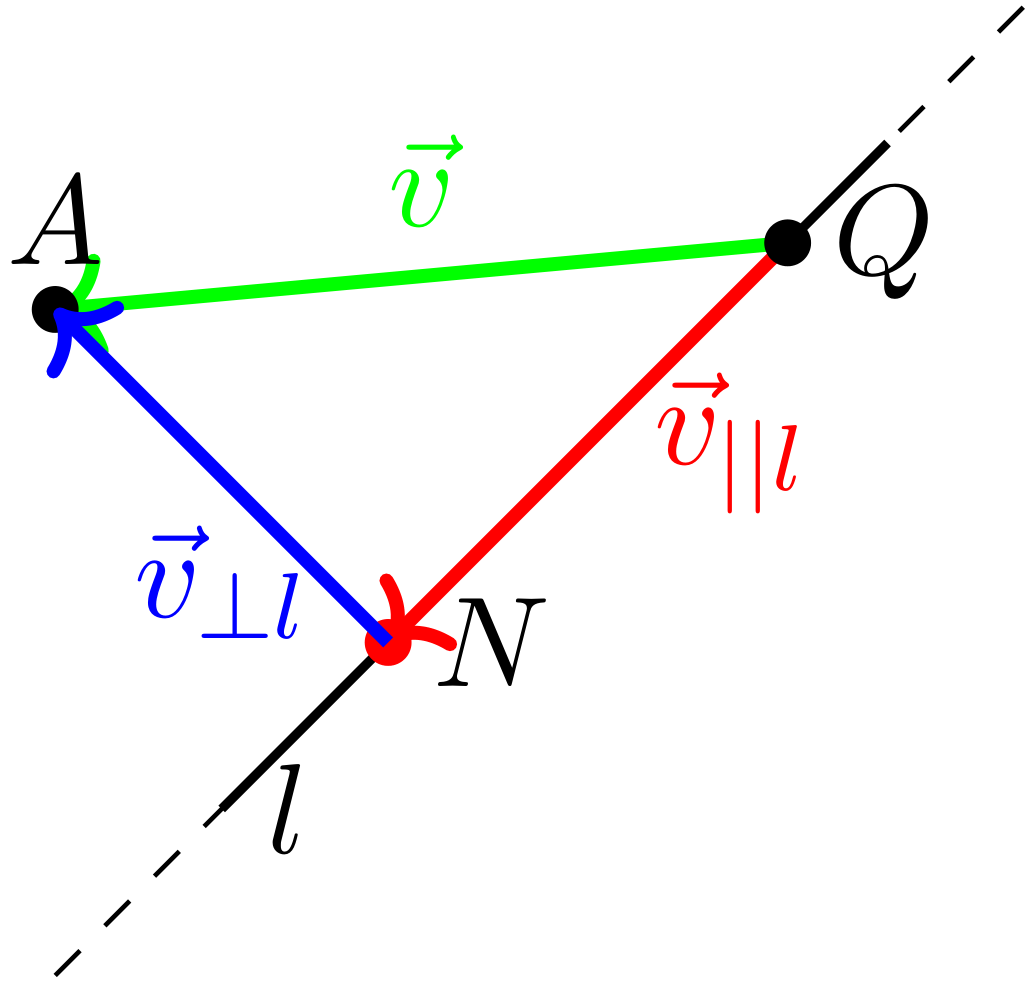
\includegraphics[width=5cm, height=5cm]{image/Ortogonal-projektion.png} 
    \caption{Ortogonal projektion}
\end{figure}

\textbf{Ortogonal projektion Formeln}
\begin{align*} 
  &\quad  \vec{v}_{||{l}} = \frac{\vec{u}\bullet{\vec{v}}}{|\vec{u}|^2}\vec{u}  \\
\end{align*}
%  &\quad  \vec{v}_{\perp{l}} = \vec{v}-\vec{v}_{||l} = \vec{v}-k\vec{u} \\

\textbf{Exempel: Hitta parralel och ortogonal komposanten}
\begin{align*} 
  &\quad  \vec{v} = \vec{v}_{\perp{l}} + \vec{v}_{||{l}} \\
  &\quad  \vec{v}_{||{l}} = \frac{\vec{u}\bullet{\vec{v}}}{|\vec{u}|^2}\vec{u}  \\
  &\quad  \text{Beräkna ortogonal komposanten av: } \\
  &\quad
  \vec{v} = \begin{pmatrix} 1 \\ -2 \\ 3 \end{pmatrix} \text{ och }
  \vec{u} = \begin{pmatrix} -4 \\ 4 \\ 2 \end{pmatrix} \\
  &\quad  \text{Beräkna först parrallel komposanten: } \\
  &\quad  \vec{v}_{||{\vec{u}}} = \frac{\vec{u}\bullet{\vec{v}}}{|\vec{u}|^2}\vec{u} = \frac{-18}{36}\vec{u}
  = \begin{pmatrix} 2 \\ -2 \\ 1 \end{pmatrix} \\
  &\quad  \text{Ortogonal komposanten blir då: } \\
  &\quad  \vec{v}_{\perp{\vec{u}}} = \vec{v} - \vec{v}_{||{\vec{u}}}
  = \begin{pmatrix} 1-2 \\ -2+2 \\ 3-1 \end{pmatrix} \\
  &\quad  \text{Svar: } \begin{pmatrix} -1 \\ 0 \\ 2 \end{pmatrix}
\end{align*}

%exempel hitta punkt
\textbf{Exempel: Närmaste punkt och avståndet}
\begin{align*} 
  &\quad  \text{Bestäm avståndet från punkten $P=(-2,4,3)$ till linjen } \\
  &\quad  \left\{\begin{array}{r}
  x+2y-z=1 \\
  x-y+5z=4 
  \end{array}\right. \\  
  &\quad  \text{Finn även den punkt på linjen l som ligger närmast punkten P}  \\
  &\quad  \\
  &\quad  \text{Skriver ekvationen på parameter form } \\
  &\quad
  \begin{gmatrix}[p]
    1 & 2  & -1 & | & 1 \\
    1 & -1 &  5 & | & 4
    \rowops{
      \add[-1]{0}{1}}
      \mult{1}{\cdot 1/3}
  \end{gmatrix} \sim{}
  \begin{gmatrix}[p]
    1 & 2  & -1 & | & 1 \\
    0 & 1 &  -2 & | & -1
    \rowops{
    \add[-2]{1}{0}}
  \end{gmatrix} \sim{}  \\
  &\quad
  \begin{gmatrix}[p]
    1 & 0  &  3 & | & 3 \\
    0 & 1 &  -2 & | & -1
    \rowops{
    \add[-1]{0}{1}}
  \end{gmatrix} \sim{}  \\
  &\quad   l:\begin{pmatrix} x \\ y \\ z \end{pmatrix} =
  \begin{pmatrix} 3 \\ -1 \\ 0 \end{pmatrix}+
  t\begin{pmatrix} -3 \\ 2 \\ 1 \end{pmatrix}  \, \text{ dvs } (p_0 + t\vec{v})\\
  &\quad  \text{Hittar en godtycklig punkt ex } t=1 \Rightarrow{}
  Q=\begin{pmatrix} 0 \\ 1 \\ 1 \end{pmatrix}  \\
  &\quad \\
  &\quad  \text{(1.) beräknar vektorn från godtykliga punkten till den givna } \\
  &\quad  \overrightarrow{PQ}=
  \begin{pmatrix} 0-(-2) \\ 1 -4 \\ 1-3 \end{pmatrix} =
  \begin{pmatrix} 2 \\ -3 \\ -2 \end{pmatrix} \\
  &\quad  \text{(2.) Beräknar ortogonala projectionen } \\
  &\quad  \overrightarrow{NQ}=\overrightarrow{PQ}_{||v}=
  \frac{\begin{pmatrix} 2 \\ -3 \\ -2 \end{pmatrix}\bullet{}
    \begin{pmatrix} -3 \\ 2 \\ 1 \end{pmatrix}}{9+4+1}
  \begin{pmatrix} -3 \\ 2 \\ 1 \end{pmatrix} =
  \frac{-14}{14}\begin{pmatrix} -3 \\ 2 \\ 1 \end{pmatrix} \\
  &\quad  \text{(3.) Beräknar punkten från närmaste punkt till } \\
  &\quad  \overrightarrow{ON}=\overrightarrow{OQ}+\overrightarrow{QN}=
  \overrightarrow{OQ}-\overrightarrow{NQ}=
  \begin{pmatrix} 0 \\ 1 \\ 1 \end{pmatrix}+
  \begin{pmatrix} -3 \\ 2 \\ 1 \end{pmatrix}=
  \begin{pmatrix} -3 \\ 3 \\ 2 \end{pmatrix} \\
  &\quad  \text{(4.) Beräknar längden }
  |\begin{pmatrix} -2 \\ 4 \\ 3 \end{pmatrix}-\begin{pmatrix} -3 \\ 3 \\ 2 \end{pmatrix}|
  =\sqrt{1^2+1^2+1^2}=\sqrt{3} \\
  &\quad  \\
  &\quad  \text{Svar: avståndet är $\sqrt{3}$ och punten är $(-3,3,2)$} \\
\end{align*}

\textbf{Exempel: Spegling}
\begin{align*} 
  &\quad  \text{Bestäm speglingen av punkten $A:(1,3,-3)$ i planet } \pi \\
  &\quad  \text{som går genom origo och innehåller punkterna}  \\
  &\quad  (-1,1,1) \text{ och } (3,3,1) \\
  &\quad  \\
  &\quad  \text{Beräknar planets ekvation} \\
  &\quad
  \vec{n}=\overrightarrow{OQ}\times\overrightarrow{OP}=
  \begin{pmatrix} -1 \\ 1 \\ 1 \end{pmatrix}\times
  \begin{pmatrix} 3 \\ 3 \\ 1 \end{pmatrix} =
  \begin{pmatrix} -2 \\ 4 \\ 6 \end{pmatrix} =
  2\begin{pmatrix} -1 \\ 2 \\ 3 \end{pmatrix} \\
  &\quad  -x+2y+3z=0 \text{ Eftersom den går egenom origo} \\
  &\quad  \overrightarrow{NA}=\overrightarrow{OA}_{||\vec{n}}=
  \frac{\begin{pmatrix} 1 \\ 3 \\ -3 \end{pmatrix}\times
    \begin{pmatrix} -1 \\ 2 \\ 3 \end{pmatrix}}{1+4+9}
  \begin{pmatrix} -1 \\ 2 \\ 3 \end{pmatrix}=
  \frac{14}{14}\begin{pmatrix} -1 \\ 2 \\ -3 \end{pmatrix} =
  \begin{pmatrix} -1 \\ 2 \\ -3 \end{pmatrix} \\
  &\quad  \text{Beräkna speglingen rita då är det upenbart } \\
  &\quad  \overrightarrow{OA'}= \overrightarrow{OA}-2\overrightarrow{NA}=
  \begin{pmatrix} 1 \\ 2 \\ -3 \end{pmatrix}-
  2\begin{pmatrix} -1 \\ 2 \\ -3 \end{pmatrix}=
  \begin{pmatrix} 3 \\ 1 \\ 3 \end{pmatrix} \\
\end{align*}


\textbf{Exempel Hitta punkt ortogonal projektion} % ex5 s12 f06
\begin{align*} 
  &\quad  \text{Låt $l$ vara linjen genom punkten $Q=(1,2,3)$ parallell med vektorn} \\
  &\quad  \vec{u} =
  \begin{pmatrix}  3 \\  4 \\  5  \end{pmatrix} \\
  &\quad  \text{Hitta den punkt $N$ på $l$ som är närmast } A=(1,7,4) \\
  &\quad  \\
  &\quad  \text{Lösning: Rita figur och tolka. Vi ortogonalt projeicerar} \\
  &\quad  \vec{v} = \overrightarrow{QA} =
  \begin{pmatrix}  1-1 \\  7-2 \\  4-3  \end{pmatrix} =
  \begin{pmatrix}  0 \\  5 \\ 1  \end{pmatrix} \text{ på vektorn }  \vec{u} \\
  &\quad \vec{v}_{||l} = \vec{v}_{||\vec{u}} = \frac{
    \begin{pmatrix} 3 \\ 4 \\ 5 \end{pmatrix} \bullet \begin{pmatrix} 0 \\ 5 \\ 1 \end{pmatrix}}{
    \begin{pmatrix} 3 \\ 4 \\ 5 \end{pmatrix} \bullet \begin{pmatrix} 3 \\ 4 \\ 5 \end{pmatrix}}
  \begin{pmatrix} 3 \\ 4 \\ 5 \end{pmatrix}
  = \frac{25}{50}\begin{pmatrix} 3 \\ 4 \\ 5 \end{pmatrix} \\
  &\quad  \text{Detta är ju igen vektorn som pekar frpn $Q$ till närmaste punkten som därför blir} \\
  &\quad  N = \Big( 1-\frac{1}{2}3, 2-\frac{1}{2}4, 3-\frac{1}{2}5 \Big)
  = \Big( -\frac{1}{2},0,\frac{1}{2} \Big) \\
  &\quad  \\
  &\quad  \text{\textbf{Kontroll:} kollar om } \overrightarrow{NQ} = k\vec{u}, \, k\in\mathbb{R} \\
  &\quad  \begin{pmatrix} 1-(-1/2) \\ 2-0 \\ 3-1/2 \end{pmatrix} =
  \begin{pmatrix} 3/2 \\ 2 \\ 5/2 \end{pmatrix} =
  \frac{1}{2}\begin{pmatrix} 3 \\ 4 \\ 5 \end{pmatrix} \text{(stämmer)} \\
\end{align*}


\textbf{Räkneregler ortogonal}
\begin{align*} 
  &\quad  \text{För vektorer $\vec{u}$, $\vec{v}$ och $\vec{w}$ och skalär $\lambda\in\mathbb{R}$} \\
  &\quad  {(\lambda\vec{v})}_{||\vec{u}}=\lambda(\vec{v}_{||\vec{u}}) \\
  &\quad  {(\vec{v}+\vec{w})}_{||\vec{u}} = \vec{v}_{||\vec{u}} + \vec{v}_{||\vec{u}} \\
  &\quad  {(\lambda\vec{v})}_{\perp{\vec{u}}} = \lambda(\vec{v}_{\perp\vec{u}}) \\
  &\quad  {(\vec{v}+\vec{w})}_{\perp{\vec{u}}} = \vec{v}_{\perp{\vec{u}}} + \vec{v}_{\perp{\vec{u}}} \\
\end{align*}


\newpage

\subsection{Enhetsvektorer och ON-baser}
\begin{align*} 
  &\quad  \text{En enhetsvektor är en vektor med längd 1.} \\
  &\quad  \text{Om man har en vektor $\vec{u}$ kan man skala om
    den med ett positivt tal så den får längd 1.} \\
  &\quad  \text{En bas } \underline{\vec{u}} = (\vec{u_1} \vec{u_2} \ldots \vec{u_n})
  \text{kallas en ortonormal bas (ON-bas) omm:} \\
  &\quad  \text{(1)  Alla vektorerna är enhetsvektorer }
  |\vec{u_1}|^2 = \vec{u_i}\bullet\vec{u_j} = 1 \\
  &\quad  \text{(2)  Varje par av vektorer $\vec{u_i}$ och $\vec{u_j}$ for $i\neq{j}$ är ortogonala:}
  \vec{u_i}\bullet\vec{u_j}=0 \\
  &\quad  \hat{\vec{u}} = \frac{1}{|\vec{u}|}\vec{u} \\
\end{align*}

Skalärproducten har samma räkneregler i ON-baser som i standard bas


\subsection{Vektorprodukten}
% https://www.youtube.com/watch?v=0GcuwYlV2ng&t=470s
I högersystem kan representeras av en höger hand där tumen är vektorn 1 pekfingret är 2
och långfingret är 3.
%bild
\textbf{Definition: högersystem}
\begin{align*} 
  &\quad  \text{En bas $\underline{u} = (\vec{u}_1 \vec{u}_2 \vec{u}_3)$
    kallas ett högersystem omm: } \\
  &\quad  \text{set ifrån spetsen av $\vec{u}_3$ vridas $\vec{u}_1$ moturs till $\vec{u}_2$} \\
\end{align*}

\textbf{Definition: Vektorprodukten}
\begin{align*} 
  &\quad  \text{Givet två icke-parallella vektorer $\vec{u}$ och $\vec{u}$ med vinkel $\theta$} \\
  &\quad  \text{mellan dem definieras $\vec{u}\times\vec{v}$ som den entydiga vektor som uppfyller} \\
  &\quad  \text{(a) } \vec{u}\times\vec{v} \text{ är ortogonal mot båda $\vec{u}$ och $\vec{v}$}  \\
  &\quad  \text{(b) längden av } \vec{u}\times\vec{v} \text{ är } |\vec{u}\vec{v}\sin{\theta}| \\
  &\quad  \text{(c) } (\vec{u} \vec{v} \vec{u}\times\vec{v}) \text{ är ett högersystem} \\
  &\quad  \text{I fallet där $\vec{u}$ och $\vec{v}$ är parallella är }
  \vec{u}\times\vec{v}=\vec{0} \\
\end{align*}

\textbf{Definition: produkter}
\begin{align*} 
  &\quad  \text{Sala om: tal $\cdot$ vektor = vektor} \\
  &\quad  \text{Skalär produkt: vektor $\bullet$ vektor = tal} \\
  &\quad  \text{Vektor produkt: vektor $\times$ vektor = vektor} \\
\end{align*}

\textbf{Räkneregler: Vektorprodukten }
\begin{align*} 
  &\quad  \text{För vektorer $\vec{u},\vec{v},\vec{w}$ och ett tal $\lambda$ gäller} \\
  &\quad  \vec{u}\times\vec{v}=-\vec{v}\times\vec{u} \\
  &\quad  \vec{u}\times(\vec{v}+\vec{w}) = \vec{u}\times\vec{v}+\vec{u}\times\vec{w}  \\
  &\quad  \lambda(\vec{u}\times\vec{v}) = \lambda(\vec{u})\times\vec{v}
  = \vec{u}\times(\lambda\vec{v}) \\
\end{align*}

\newpage
\textbf{Vektorprodukten metologi}
\begin{figure}[h]
    \vspace{10mm}
    \centering
    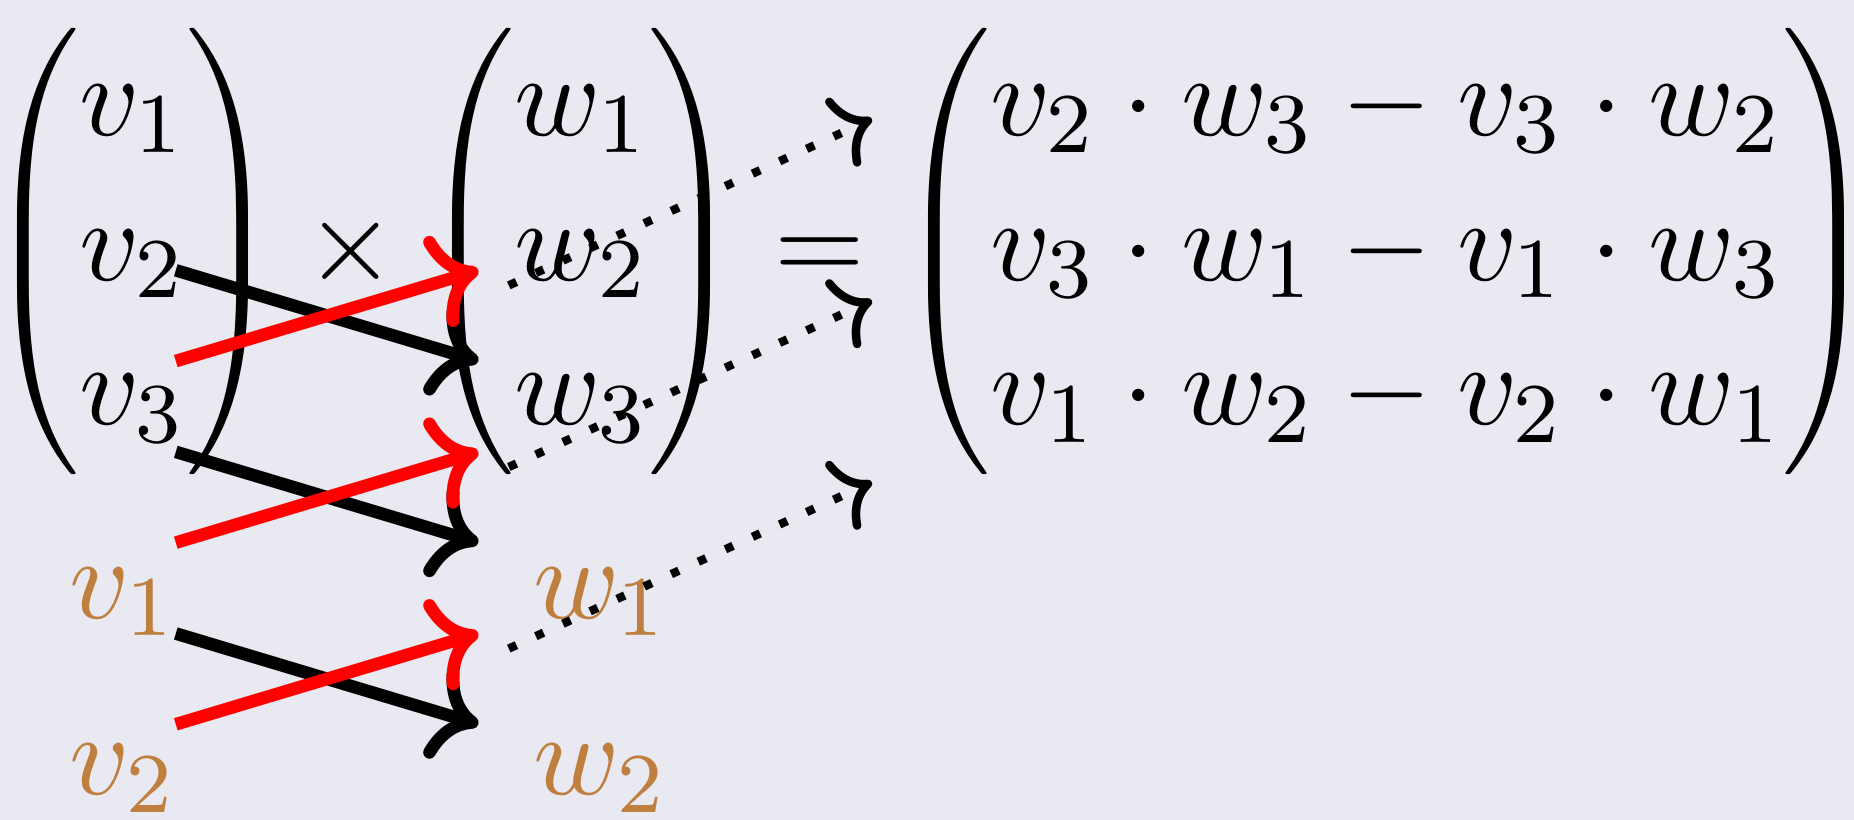
\includegraphics[width=12cm, height=5cm]{image/vektorprodukt.png} 
    \caption{Vektorprodukten}
\end{figure}

\textbf{Exempel: Hitta basen}
\begin{align*} 
  &\quad  \text{Låt }
  \vec{u}_1 = \begin{pmatrix} 4 \\ 8 \\ 1 \end{pmatrix} \text{ och }
  \vec{u}_2 = \begin{pmatrix} 4 \\ -1 \\ -8 \end{pmatrix} \\
  &\quad  \text{Verifiera att dessa är ortogonala, och hitta en vektor } \vec{u}_3 \\
  &\quad  \text{Så att } \underline{u} = (\hat\vec{u}_1 \hat\vec{u}_2 \hat\vec{u}_3)
  \text{ är en ON-bas (och skriv ut denna)} \\
  &\quad  \\
  &\quad  \text{Lösning: Först kollar vi att skalärprodukten är } 0: \\
  &\quad
  \begin{pmatrix} 4 \\ 8 \\ 1 \end{pmatrix} \bullet \begin{pmatrix} 4 \\ -1 \\ -8 \end{pmatrix}
  = 16-8-8=0 \\
  &\quad  \text{Där med ortogonala. Nu måste vi hitta en vektor som är ortogonal mot båda } \\
  &\quad  \text{vektorprodukten är just det } \\
  &\quad  \vec{u}_3 =
  \begin{pmatrix} 4 \\ 8 \\ 1 \end{pmatrix} \times \begin{pmatrix} 4 \\ -1 \\ -8 \end{pmatrix}
  \begin{pmatrix} -64+1 \\ 4+32 \\ -4-32 \end{pmatrix} =
  \begin{pmatrix} -63 \\ 36 \\ -36 \end{pmatrix} \\
  &\quad  \text{Längderna av dessa är (råkar vara lika)}  \\
  &\quad  |\vec{u}_2|^2 = |\vec{u}_1|^2 = 4^2 + {(\pm{8})}^2 + {(\pm{1})}^2 = 81 \\
  &\quad  \text{och vi kunna göra liknade beräkning för } \vec{u}_3 \text{, men vi vet redan att:} \\
  &\quad  |\vec{u}_3| = |\vec{u}_1||\vec{u}_2|\sin{\theta}=9\cdot{}9\cdot{}1=81 \\
  &\quad  \text{Desras tre normering blir därför:} \\
  &\quad  \hat\vec{u}_1 = \frac{1}{9}\begin{pmatrix} 4 \\ 8 \\ 1 \end{pmatrix},
  \hat\vec{u}_2 = \frac{1}{9}\begin{pmatrix} 4 \\ -1 \\ -8 \end{pmatrix}
  \hat\vec{u}_1 = \frac{1}{81}\begin{pmatrix} -63 \\ 36 \\ -36 \end{pmatrix}=
  \frac{1}{9}\begin{pmatrix} -7 \\ 4 \\ -4 \end{pmatrix} \\
  &\quad  \text{Så basen är: }
  \underline{u} = \Bigg(
  \frac{1}{9}\begin{pmatrix} 4 \\ 8 \\ 1 \end{pmatrix},
  \frac{1}{9}\begin{pmatrix} 4 \\ -1 \\ -8 \end{pmatrix},
  \frac{1}{81}\begin{pmatrix} -63 \\ 36 \\ -36 \end{pmatrix}
  \Bigg) \\
\end{align*}

\textbf{Exempel: Uttryck vektorer i varandra (2.5.8.b)}
\begin{align*}
  &\quad  \text{Uttryck $w$ i $u$ och $v$} \\
  &\quad  |u|=6, \, |v|=8, |w|=7, \text{ $u$ och $v$ bildar vinkeln } \frac{\pi}{6}, \\
  &\quad  \text{ $u$ och $w$ vinkeln } \frac{\pi}{2} \text{ och $v$ och $w$ vinkeln } 
  \frac{2\pi}{3}  \\
  &\quad  \\
  &\quad  \text{Altså ska hitta } \vec{w}=k_1\vec{u}+k_2\vec{v}, \, k_1,k_2\in\mathbb{R} \\
  &\quad  \text{Vi ser att $k_2<0$ enlight bild, därmed får vi följande } \\
  &\quad  -k_2\cdot\cos{\frac{\pi}{3}}=7 \Rightarrow -k_2\cdot{\frac{1}{2}}\cdot{8}=7
  \Rightarrow k_2=\frac{7}{4} \\
  &\quad  \text{Beräknarn $k_1$ } \\
  &\quad  6k_1=\frac{7}{4}\cdot{8}\cdot{\sin{\frac{\pi}{3}}} \Rightarrow k_1=\frac{7}{6}\sqrt{3} \\
  &\quad  \vec{w}=\frac{7\sqrt{3}}{6}\vec{u}-\frac{7}{4}\vec{v} \\
\end{align*}
\begin{figure}[h]
    \vspace{10mm}
    \centering
    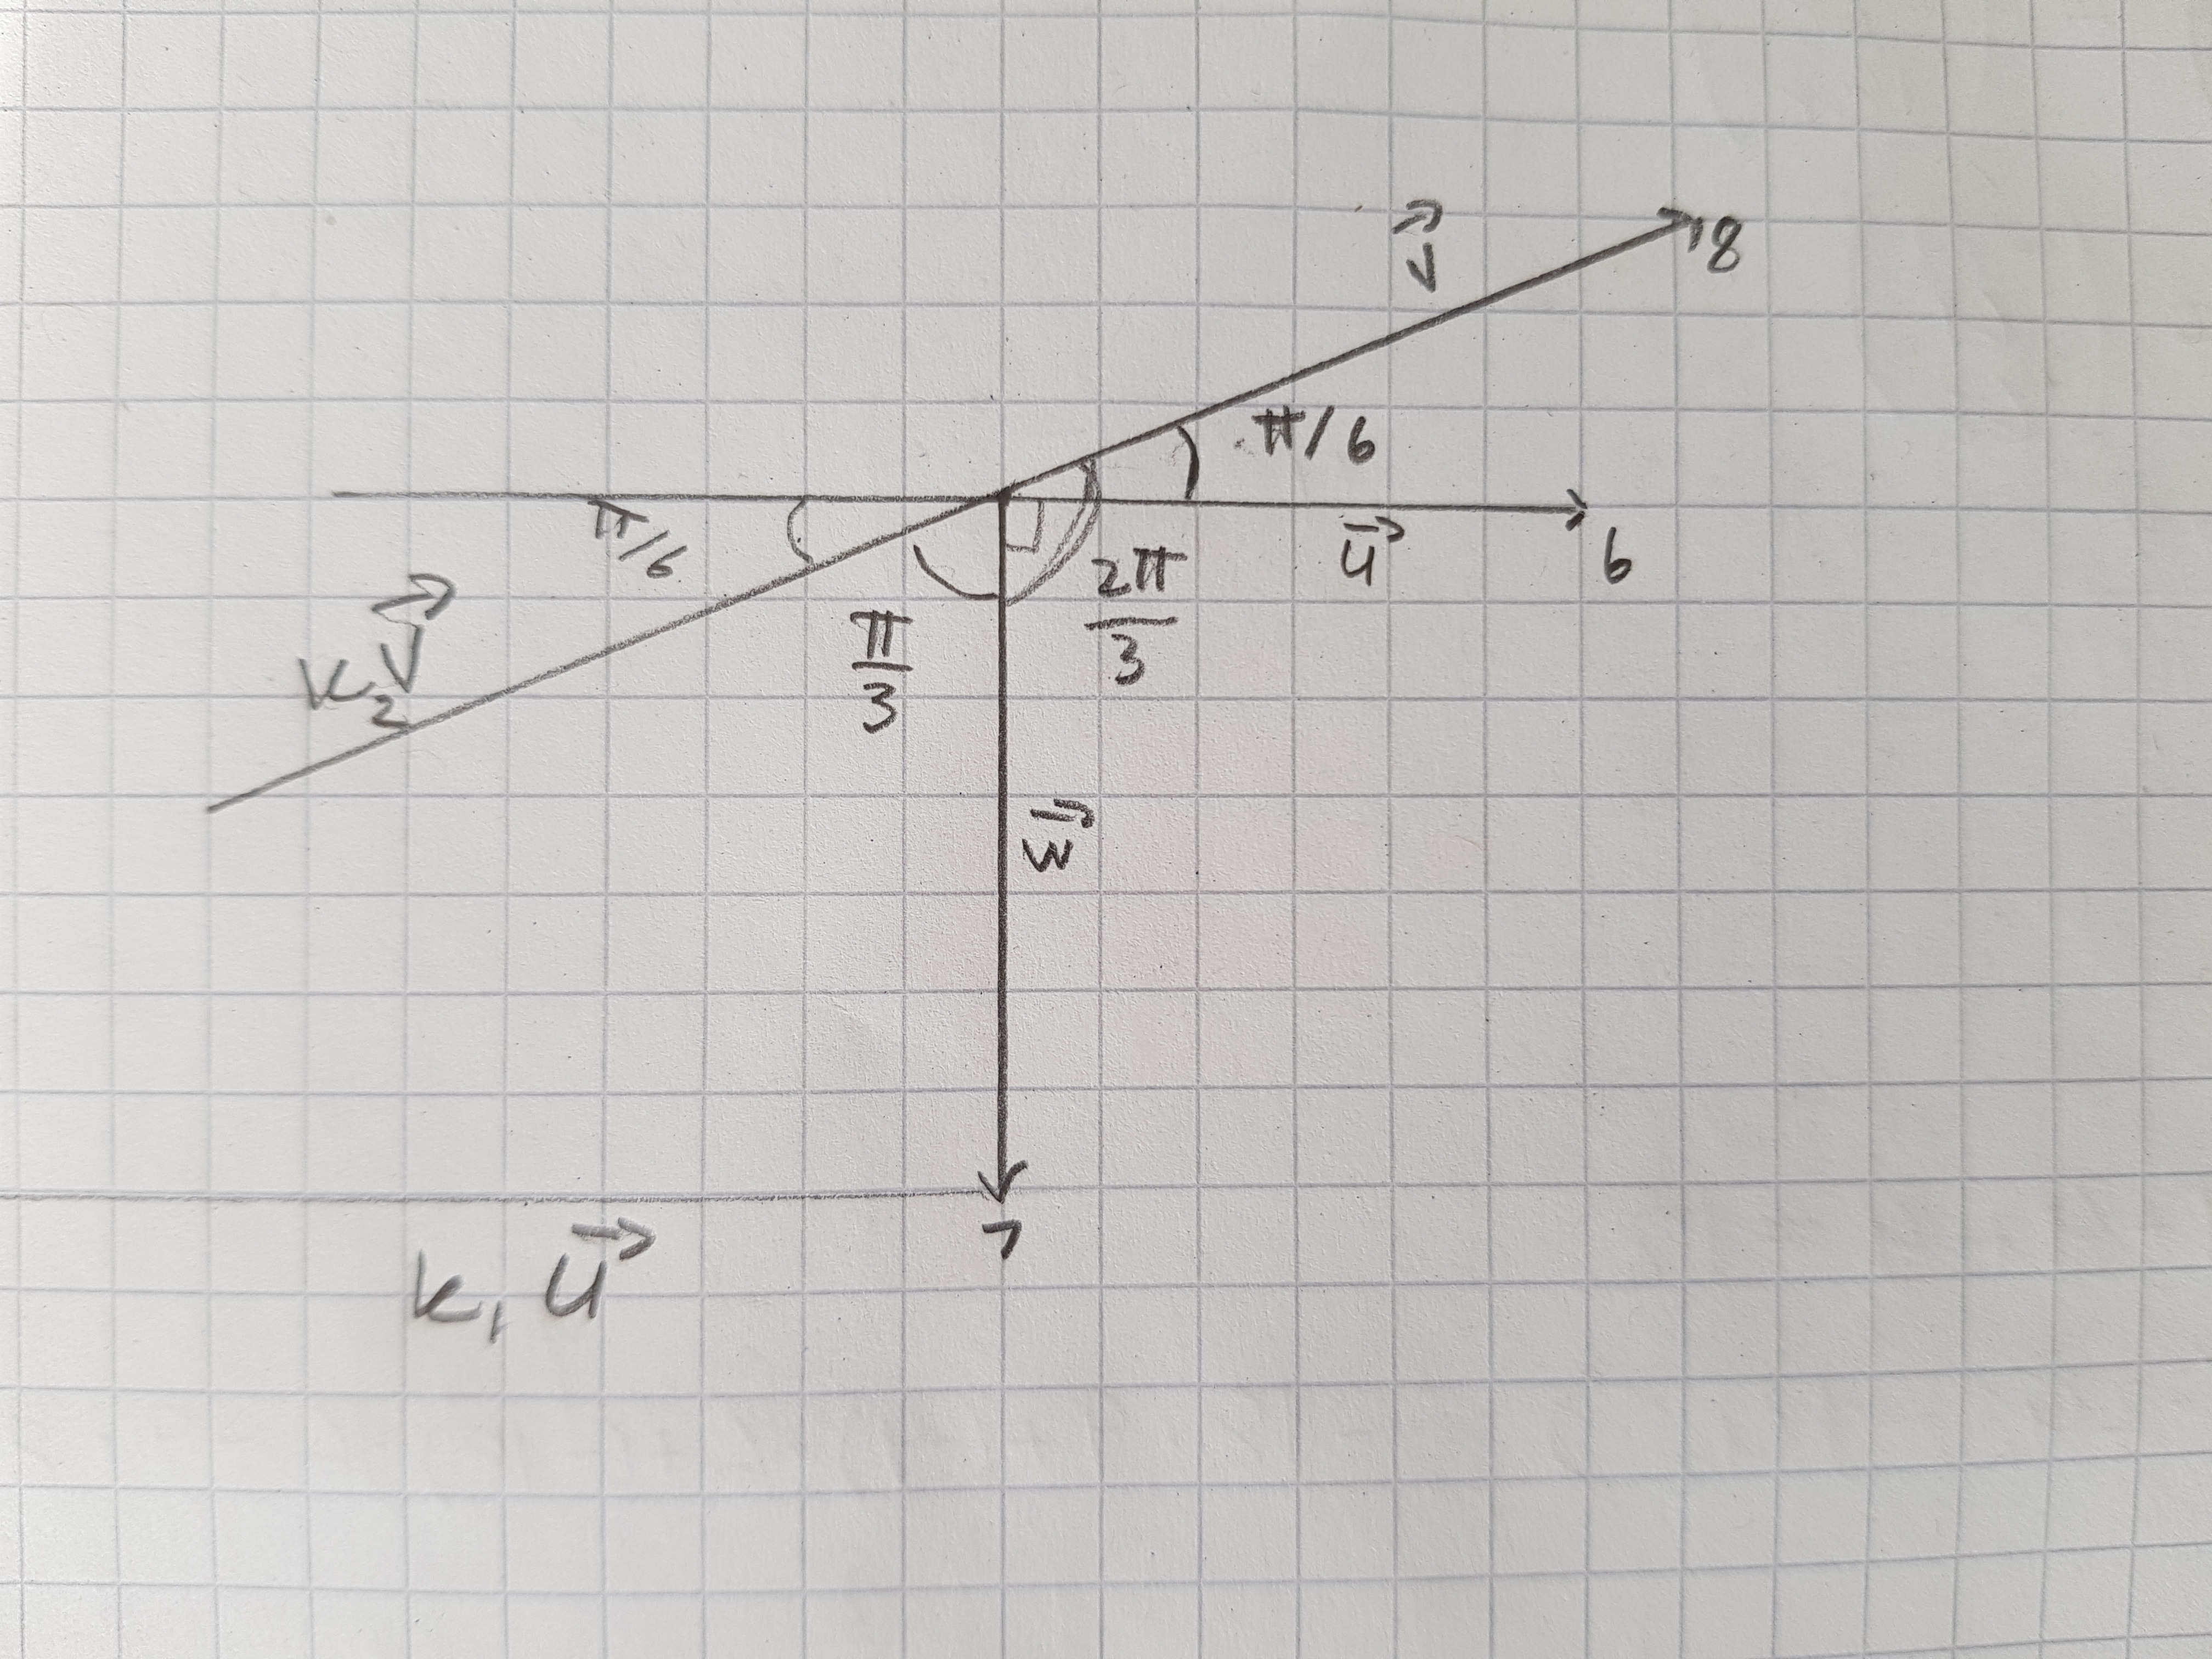
\includegraphics[width=10cm, height=6cm]{image/2.5.8.b.jpg} 
    \caption{2.5.8.b}
\end{figure}


\newpage

\subsection{Area och Volym}
%\textbf{Vektorprodukten räkneregler}
\begin{align*} 
  &\quad  \text{Area parralelogram: } |\vec{u}||\vec{v}|\sin{\theta} = |\vec{u}\times\vec{v}| \\
  &\quad  \text{Volym parralelogram: } |(\vec{u}\times\vec{v})\bullet\vec{w}|
\end{align*}

\begin{figure}[h]
    \vspace{10mm}
    \centering
    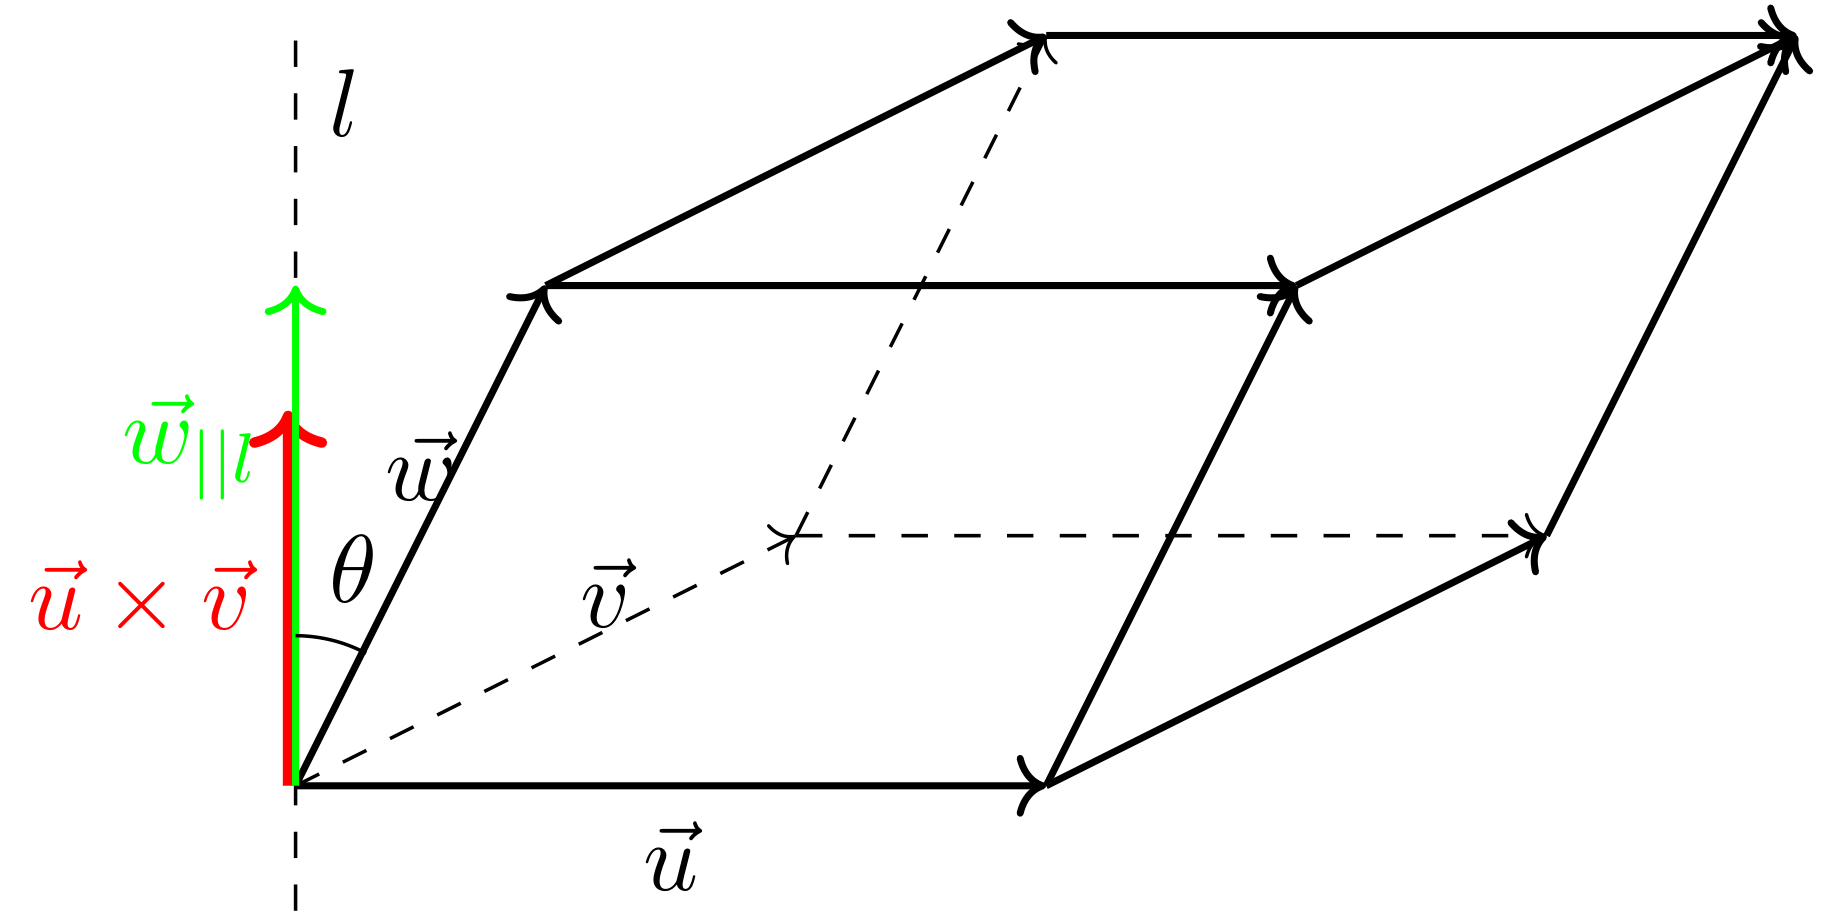
\includegraphics[width=11cm, height=6cm]{image/parallelogram.png} 
    \caption{Ortogonal projektion}
\end{figure}

\textbf{Exempel: Hitta volymen}
\begin{align*} 
  &\quad  \text{Hitta volymen av parallellipipeden med sidorna } \\
  &\quad
  \vec{u} = \begin{pmatrix} 1 \\ 1 \\ 1 \end{pmatrix}
  \vec{v} = \begin{pmatrix} 2 \\ 1 \\ 1 \end{pmatrix}
  \vec{w} = \begin{pmatrix} 1 \\ 1 \\ 2 \end{pmatrix} \\
  &\quad  \text{och avgör om $(\vec{u} \vec{v} \vec{w})$ är ett högersystem,} \\
  &\quad  \text{ett vänstersystem, eller ej en bas.} \\
  &\quad  \\
  &\quad  \text{Lösning: Vi beräknar} \\
  &\quad  \vec{u}\times\vec{v} =
  \begin{pmatrix} 1\cdot{1}-1\cdot{1} \\ 1\cdot{2}-1\cdot{1} \\ 1\cdot{1}-1\cdot{2} \end{pmatrix}
  = \begin{pmatrix} 0 \\ 1 \\ -1 \end{pmatrix} \\
  &\quad  (\vec{u}\times\vec{v})\bullet\vec{w} = 0+1-2=-1 \\
  &\quad  \text{Så det är ett vänstersystem och volymen är 1} \\
\end{align*}


\newpage

\section{Linjer och plan}
\begin{align*} 
  &\quad  \text{Parameterform: }
  \begin{pmatrix} x \\ y \\ z \end{pmatrix} =
  \begin{pmatrix} a_1 \\ a_2 \\ a_3 \end{pmatrix} +
  t\begin{pmatrix} v_1 \\ v_2 \\ v_3 \end{pmatrix}, t \in\mathbb{R} \\
  &\quad  \text{Normalform: } ax+by=c \Rightarrow
  \vec{n} = \begin{pmatrix} a \\ b \end{pmatrix} \\
  &\quad  \text{Plan: }
  \begin{pmatrix} x \\ y \\ z \end{pmatrix} =
  \begin{pmatrix} p_1 \\ p_2 \\ p_3 \end{pmatrix} +
  t\begin{pmatrix} u_1 \\ u_2 \\ u_3 \end{pmatrix} +
  s\begin{pmatrix} v_1 \\ v_2 \\ v_3 \end{pmatrix} \\
\end{align*}


\textbf{Exempel: Skriv i parameterform}
\begin{align*} 
  &\quad  \text{Om vi lösar ekvationen (vars lösningar är en linje): } x+3y=4; \\
  &\quad  y=t \Rightarrow x=4-3t \Rightarrow 
  \begin{pmatrix} x \\ y \end{pmatrix} =
  \begin{pmatrix} 4 \\ 0 \end{pmatrix} +
  t\begin{pmatrix} -3 \\ 1 \end{pmatrix} \\
  &\quad  \text{Hitta parameterform för linje genom givna punkter} \\
  &\quad 
  A= \begin{pmatrix} -21 \\ 20 \end{pmatrix},
  B= \begin{pmatrix} -24 \\ -22 \end{pmatrix} \\
  &\quad  \overline{AB} = \overline{OB}-\overline{0A} =
  \begin{pmatrix} -24-(-21) \\ -22-20 \end{pmatrix} =
  \begin{pmatrix} -3 \\ -42 \end{pmatrix} \Rightarrow \\
  &\quad  L:\underline{e}\begin{pmatrix} x \\ y \end{pmatrix} =
  \underline{e}\begin{pmatrix} -21 \\ 20 \end{pmatrix} +
  t\underline{e}\begin{pmatrix} -3 \\ -42 \end{pmatrix} \\
\end{align*}


\textbf{Exempel: Hitta planets ekvation}
\begin{align*}
  &\quad  \text{Uppgift: Hitta en ekvation för planet som } \\
  &\quad  \text{går genom $(1, 2, 3)$ och är parallell med vektorna } \\
  &\quad
  \vec{u} = \begin{pmatrix} 4 \\ 5 \\ 6 \end{pmatrix}
  \vec{v} = \begin{pmatrix} 7 \\ 8 \\ 9 \end{pmatrix} \\
  &\quad  \\
  &\quad  \text{Lösnig: Vi måste hitta en vektorn $\vec{n}$ som är ortogonal mot planet}  \\
  &\quad  \text{Inte så lätt i 3D som för linje i 2D. Men vi har en formel.} \\
  &\quad
  \vec{n} = \begin{pmatrix} 4 \\ 5 \\ 6 \end{pmatrix} \times
  \begin{pmatrix} 7 \\ 8 \\ 9 \end{pmatrix} =
  \begin{pmatrix} 45-48 \\ 42-36 \\ 32-35 \end{pmatrix} =
  \begin{pmatrix} -3 \\ 6 \\ -3 \end{pmatrix} \\
  &\quad  \text{Det kan vi skriva på normal formen: }
  -3x+6y-3z=c \\
  &\quad  \text{För att hitta $c$ så insätter vi det kända punkten $(1,2,3)$} \\
  &\quad  c = -3\cdot{1}+6\cdot{2}-3\cdot{3} = 0 \\
  &\quad  \text{Vi får formen: } -3x+6y-3z=0 \\
\end{align*}


\textbf{Exempel: Beskriva linje på normalform} 
\begin{align*} %https://www.youtube.com/watch?v=kam3foz8eqA
  &\quad  \text{Uppgift: Hitta normalvektorn för linje } A=(16,4), B=(9,12) \\
  &\quad  \overline{AB} = 
  \begin{pmatrix} 9-16 \\ 12-4 \end{pmatrix} = \begin{pmatrix} -7 \\ 8 \end{pmatrix} \\
  &\quad  L: \overline{OA}+t\overline{AB}=
  \begin{pmatrix} 16 \\ 4 \end{pmatrix} + t\begin{pmatrix} -7 \\ 8 \end{pmatrix} \\
  &\quad  \left\{\begin{array}{r}
  x=16-7t \\
  y=4+8t  
  \end{array}\right. \\
  &\quad  t=\frac{16-x}{7}=\frac{y-3}{8} \Leftrightarrow{} 128 -8x=7y-21 \\
  &\quad  8x+7y=149 \\
\end{align*}
%  &\quad  \text{Uppgift: Hitta normalvektorn för plan} \\

\textbf{Exempel: Skärning mellan plan} %https://www.youtube.com/watch?v=DrD4mBq6_4Q
\begin{align*} %% antat exempel
  &\quad  \left\{\begin{array}{r}
  -3x+y+4z=4 \\
  x-4y-5z=-5 
  \end{array}\right. \\
  &\quad  \\
  &\quad  \left\{\begin{array}{r}
  0-11y-11z=-11 \\
  x-4y-5z=-5 
  \end{array}\right. \\
  &\quad  \left\{\begin{array}{r}
  0+y+z=1 \\
  x-4y-5z=-5 
  \end{array}\right. \\
  &\quad  \left\{\begin{array}{r}
  x+0-z=-1 \\
  0+y+z=1 
  \end{array}\right. \\
  &\quad  \begin{pmatrix} t-1 \\ 1-t \\ t \end{pmatrix} \\
\end{align*}


\textbf{Exempel: Skärning mellan plan och linjen} %https://www.youtube.com/watch?v=Av0wOqkLojU
\begin{align*} %% antat exempel
  &\quad  3x+3y+4z=-7 \\
  &\quad  \left\{\begin{array}{r}
  x = 2-3t \\
  y = 1-3t \\
  z = 3t
  \end{array}\right. \\
  &\quad  3(2- 3t)+3(1 -3t)+4(3t)=-7 \Rightarrow{} -6t=-16  \Rightarrow{} t=\frac{8}{3} \\
  &\quad  \left\{\begin{array}{r}
  x = 2-3t = -6 \\
  y = 1-3t = -7 \\
  z = 3t = 8 
  \end{array}\right. \\
\end{align*}



\newpage

\subsection{ortogonal projektion på plan}
\begin{figure}[h]
    \vspace{10mm}
    \centering
    \includegraphics[width=14cm, height=6cm]{image/ortogonal_projektion_på_plan.png} 
    \caption{Ortogonal projektion på plan}
\end{figure}

\textbf{Exempel: Hitta närmaste punkten i planet} %https://www.youtube.com/watch?v=749xxpKLvzQ
\begin{align*}
  &\quad  \text{Uppgift: hitta närmaste punkten $N$ till punkten } A = (1,-5,2) \\
  &\quad  \text{i planet } P: x+2y-z=1 \text{ Hitta även avståndet mellan $A$ och planet} \\
  &\quad  \\
  &\quad  \text{Lösning: Först väljer vi godtycklig punkt } Q=(1,0,0)
  \text{ i planet, och beräknar} \\
  &\quad  \vec{v}=\overrightarrow{QA} =
  \begin{pmatrix} 1-1 \\ -5 \\ 2 \end{pmatrix} =
  \begin{pmatrix} 0 \\ -5 \\ 2 \end{pmatrix} \\
  &\quad  \text{Normalvektor till planet } x+2y-z=1
  \vec{n} = \begin{pmatrix} 1 \\ 2 \\ -1 \end{pmatrix} \\
  &\quad  \vec{v}_{||\vec{n}} = \frac{0\cdot{1}+(-5)\cdot{2}+2\cdot{(-1)}}{1^2+2^2+{(-1)}^2}\vec{n}
  = -2\vec{n} \\
  &\quad  \text{Så vi får koordinaterna: } \\
  &\quad  \overrightarrow{ON} = \overrightarrow{OA} - \overrightarrow{AN}
  = \overrightarrow{OA}-\vec{v}_{||\vec{n}} =
  \begin{pmatrix} 1 \\ -5 \\ 2 \end{pmatrix} - (-2)\vec{n} =
  \begin{pmatrix} 3 \\ -1 \\ 0 \end{pmatrix} \\
  &\quad  \text{så närmaste punkten är $N = (3,-1,0)$ Avståndet är } |-2\vec{n}| = 2\sqrt{6} \\
\end{align*}

\textbf{Exempel: Hitta närmaste punkten på linje till linje} %F10
\begin{align*}
  &\quad  \text{Hitta den punkt på linjen } \\
  &\quad  
  l: \begin{pmatrix} x \\ y \\ z \end{pmatrix} = \begin{pmatrix} -1 \\ 0 \\ 0 \end{pmatrix} +
  t\begin{pmatrix} 1 \\ 1 \\ 1 \end{pmatrix}, \, t\in\mathbb{R} \\
  &\quad  \text{som är närmast linjen } \\
  &\quad
  k: \begin{pmatrix} x \\ y \\ z \end{pmatrix} = \begin{pmatrix} -1 \\ 0 \\ -1 \end{pmatrix} +
  s\begin{pmatrix} 1 \\ 2 \\ 1 \end{pmatrix}, \, s\in\mathbb{R} \\
  &\quad  A=(-1+t,t,t), \, B=(-1+s,2s,-1+s) \\
  &\quad  \overrightarrow{AB}=
  \begin{pmatrix} (-1+s)-(-1+t) \\ (2s)-(t) \\ (-1+s)-(t) \end{pmatrix} =
  \begin{pmatrix} s-t \\ 2s-t \\ -1+s-t \end{pmatrix} \\
  &\quad  \text{Vektorn ska vara ortogonal mot: }
  \begin{pmatrix} 1 \\ 1 \\ 1 \end{pmatrix} \land
  \begin{pmatrix} 1 \\ 2 \\ 1 \end{pmatrix} \\
  &\quad
  \left\{\begin{array}{r}
  1(s-t) + 1(2s-t) + 1(-1+s-t) = 0  \\
  1(s-t) + 2(2s-t) + 1(-1+s-t) = 0  
  \end{array}\right. =
  \left\{\begin{array}{r}
  -1 + 4s + -3t = 0  \\
  -1 + 6s + -4t = 0 
  \end{array}\right. \\
  &\quad  \Rightarrow{} s=\frac{3t+1}{4} \Rightarrow{} -1 + \frac{3}{2} (3t+1) -4t = 0 \\
  &\quad 
  \left\{\begin{array}{r}
  t=-1  \\
  s=-1/2
  \end{array}\right. \text{(Kontrollera)} -1 -2 +3 = 0, \, -1 -3 +4 = 0 \\
  &\quad  A= (-2,-1,-1), \, B= (-3/2,-1,-3/2)  \Rightarrow\overrightarrow{AB}=
  \begin{pmatrix} 1/2 \\ 0 \\ -1/2 \end{pmatrix} \\
  &\quad  \text{Svar: punkten på linjen $l$ är } A= (-2,-1,-1) \\
\end{align*}


\newpage

\section{Matrisräkning}
\textbf{Begräpp: matriser}
\begin{align*} 
  &\quad  \text{diagonal} \\
  &\quad  \text{huvuddiagonalen} \\
  &\quad  \text{Kummuterar: } AB=BA \\
  &\quad  A={(a_{ij})}_{r\times{k}} \\
  &\quad  \text{Rang: antalet ledande kofisent i trappsteksmatris } \\ 
\end{align*}

\textbf{Räkneregler: matriser}
\begin{align*}
  &\quad  \text{Addition: endast i sama form} \\
  &\quad  \text{Multiplication: } (r\times{k})(k\times{m}) \Rightarrow r\times{x}  \\
  &\quad  (AB)C=A(BC) \\
  &\quad  \lambda(AB) = (\lambda{A})B = A(\lambda{B}) \\
  &\quad  A(B+C) = AB + AC \\
  &\quad  (B+C)A = BA+CA \\
\end{align*}

\begin{figure}[h]
    \vspace{10mm}
    \centering
    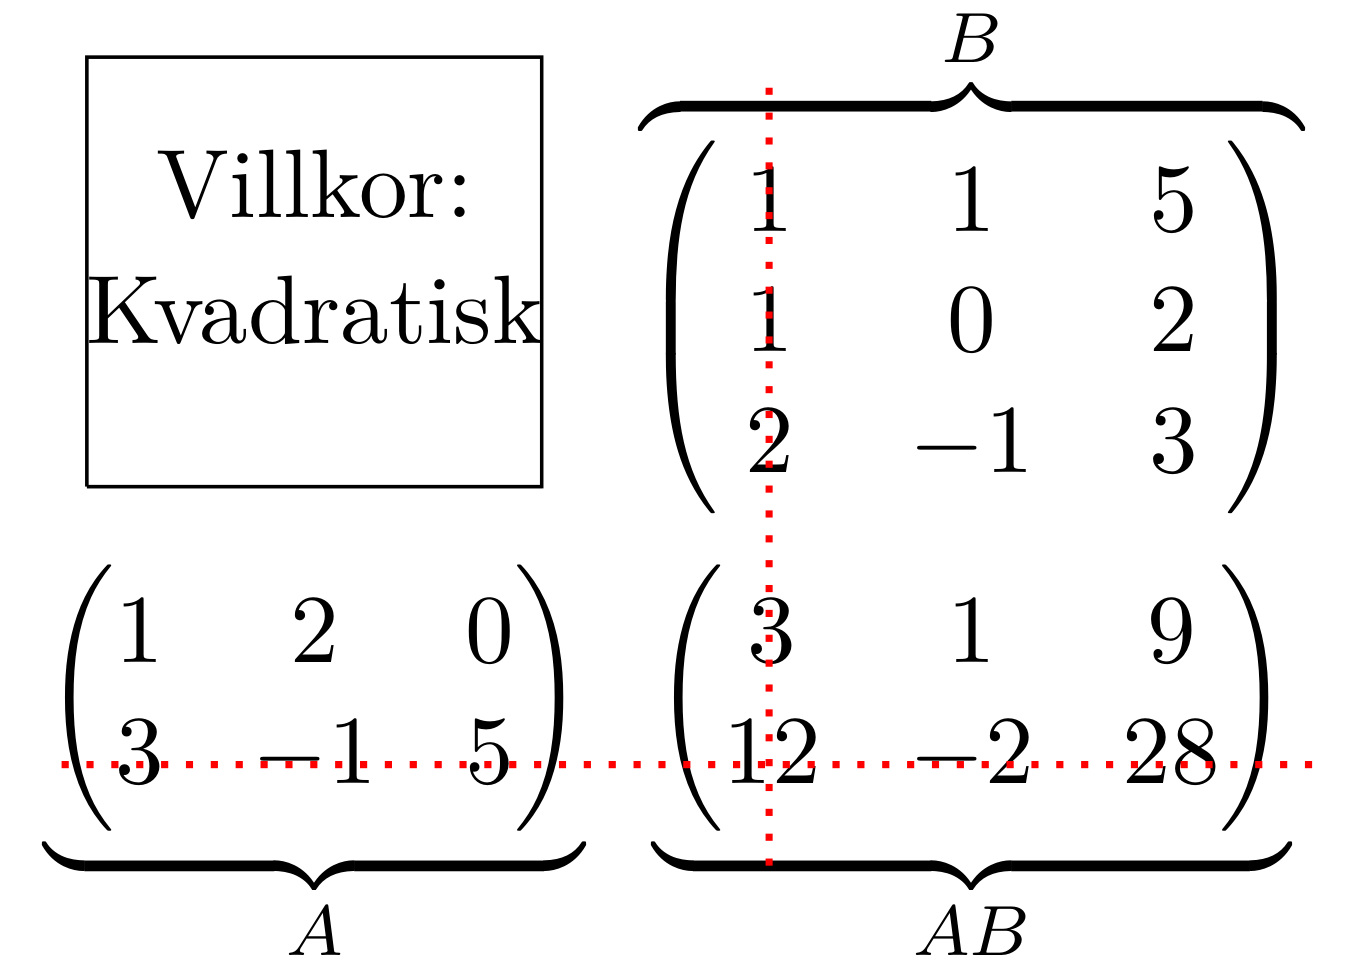
\includegraphics[width=10cm, height=6cm]{image/matris-multiplikation.png} 
    \caption{Ortogonal projektion på plan}
\end{figure}

\textbf{Exempel: Multiplication av matriser}
\begin{align*}
  &\quad
  \left(\begin{array}{ccc}
    2  & 3  & 4 \\
    -1 & 2  & 2 \\
    -5 & -2 & 1 
  \end{array}\right)
  \left(\begin{array}{c}
    a \\
    b \\
    c 
  \end{array}\right) =
  \left(\begin{array}{ccc}
    2a  & 3b  & 4c \\
    -a & 2b  & 2c \\
    -5a & -2b & c 
  \end{array}\right)
\end{align*}

\textbf{Definition: Enhetsmatrisen}
\begin{align*}
  &\quad  \text{Enhetsmatrisn } I_n \\
  &\quad  A^0I_n = I_n \\
  &\quad  A: 2\times{2} AI_2 = A \\
  &\quad  I_3 =
  \left(\begin{array}{ccc}
    1 & 0 & 0 \\
    0 & 1 & 0 \\
    0 & 0 & 1 
  \end{array}\right)
\end{align*}


\subsection{Transpornat}
\textbf{Definition: Transponaten}
\begin{align*}
  &\quad  A^t \text{ betyder inte A upphöjt till t} \\
  &\quad  A={(a_{ij})}_{r\times{k}} \Rightarrow A^t=A={(\alpha_{ij})}_{k\times{r}} \\
  &\quad  A={(\alpha_{ij})}={(a_{ij})}  \\
\end{align*}

\textbf{Exempel: Transponaten}
\begin{align*}
  &\quad  \text{Symetrisk } A=A^t \\
  &\quad
  \left(\begin{array}{cccc}
    1 & 2 & 3 & 4 \\
    5 & 6 & 7 & 8
  \end{array}\right)^t =
  \left(\begin{array}{cc}
    1 & 5 \\
    2 & 6 \\
    3 & 7 \\
    4 & 8
  \end{array}\right)
\end{align*}

\textbf{Räkneregler: Transponaten}
\begin{align*}
  &\quad  {(A+B)}^t = A^t+B^t \\
  &\quad  {(\lambda A)}^t = \lambda A^t \\
  &\quad  {(A^t)}^t = A \\
  &\quad  {(AB)}^t = B^t A^t \\
\end{align*}


\subsection{Matrisinvers}
% X=X_p+X_h
\textbf{Räkneregler: Matrisinvers }
\begin{align*}
  &\quad  AB=BA=I \\
  &\quad  \text{Inversen finns endast om matrisen är kvadratisk} \\
  &\quad  A \text{ är inventerba} \\
  &\quad  AX=B \text{ har entydiga lösningar för alla B} \\
  &\quad  AX=0 \text{ har enbart lösningen} X=0 \\
  &\quad  A \text{ har rang} n \\
  &\quad  A \sim I  \text{ (är radekvivalent med) } I
\end{align*}

\textbf{Exempel: Matrisinvers 3x3}
\begin{align*}
  &\quad
  \left(\begin{array}{ccc}
    1 & 2 & 1 \\
    1 & 1 & 0 \\
    0 & 1 & -1 \\
  \end{array}\right) \sim{}
  \left(\begin{array}{ccc|ccc}
    1 & 2 & 1   & 1 & 0 & 0 \\
    1 & 1 & 0   & 0 & 1 & 0 \\
    0 & 1 & -1  & 0 & 0 & 1 \\
  \end{array}\right) \sim{}
  \left(\begin{array}{ccc|ccc}
    1 & 2  & 1  & 1  & 0 & 0 \\
    0 & -1 & -1 & -1 & 1 & 0 \\
    0 & 1  & -1 & 0  & 0 & 1 \\
  \end{array}\right) \sim{} \\
  &\quad
  \left(\begin{array}{ccc|ccc}
    1 & 0  & -1 & -1  & 2    & 0   \\
    0 & 1  & 1  & 1   & -1   & 0   \\
    0 & 1  & 1  & 1/2 & -1/2 & -1/2 \\
  \end{array}\right) \sim{}
  \left(\begin{array}{ccc|ccc}
    1 & 0  & 0  & -1/2  & 3/2  & -1/2   \\
    0 & 1  & 0  & 1/2   & -1/2 & 1/2 \\
    0 & 0  & 1  & 1/2   & -1/2 & -1/2 \\
  \end{array}\right) \sim{} \\
  &\quad
  A^{-1}=
  \left(\begin{array}{ccc}
    -1/2  & 3/2  & -1/2   \\
    1/2   & -1/2 & 1/2 \\
    1/2   & -1/2 & -1/2 \\
  \end{array}\right) = \frac{1}{2}
  \left(\begin{array}{ccc}
    -1  & 3  & -1  \\
    1   & -1 & 1   \\
    1   & -1 & -1  \\
  \end{array}\right)
\end{align*}

\textbf{Räkneregler: Matrisinvers }
\begin{align*}
  &\quad  A =
  \left(\begin{array}{cc}
    a & b  \\
    c & d  \\
  \end{array}\right) \\
  &\quad  A^{-1} = \frac{1}{ad-bc} 
  \left(\begin{array}{cc}
    d  & -b  \\
    -c & a  \\
  \end{array}\right) \\
\end{align*}

%vissa hur man gör kontrolera på exemplerna

\newpage

\section{Determinanter}
Ekvations system har unika lösningar då koefficient matrisen är inventerbar.
Som är ekvivalent med att determinanten är nollskild.

\textbf{Exempel: determinant många led genväg }
\begin{align*}
  &\quad  
  \left(\begin{array}{ccccc}
    3 & 2 & -3 & 24 & 1005 \\
    0 & 1 & 23 & 14 & 15 \\
    0 & 0 & 3  & 7  & -5 \\
    0 & 0 & 2  & 4  & 3 \\
    0 & 0 & 0  & 0  & 5 \\
  \end{array}\right) \\
  &\quad \text{Vi det finns endast två producter som inte inehåller en nol faktor} \\
  &\quad
  \left(\begin{array}{ccccc}
    (3) & 2 & -3 & 24 & 1005 \\
    0 & (1) & 23 & 14 & 15 \\
    0 & 0 & (3)  & (7)  & -5 \\
    0 & 0 & (2)  & (4)  & 3 \\
    0 & 0 & 0  & 0  & (5) \\
  \end{array}\right) = 3\cdot{1}\cdot{3}\cdot{4}\cdot{5}-3\cdot{1}\cdot{6}\cdot{2}\cdot{5}=0
\end{align*}

\textbf{Exempel: determinant 3x3 }
\begin{align*}
  &\quad  
  \left(\begin{array}{ccc}
    1 & 2 & 3  \\
    4 & 5 & 6  \\
    7 & 8 & 9
  \end{array}\right) = \\
  &\quad  =1\cdot{5}\cdot{9}-1\cdot{6}\cdot{8}-2\cdot{4}\cdot{9}+ \\
  &\quad  +2\cdot{6}\cdot{7}+3\cdot{4}\cdot{8}-3\cdot{5}\cdot{7}= \\
  &\quad  =45-48-72+84+96-105=0 \\
\end{align*}

\textbf{Sats:}
\begin{align*}
  &\quad   \text{Om $B$ är matrisen $A$ där man har bytt om på rad $i$ och $j$ är } detA = -detB \\
  &\quad   (1) \text{ Bytt två rader om i $A$ ändras determinaten sitt teken} \\
  &\quad   (2) \text{ Skalas en rad om med $\lambda$ skalas också determinaten om med } \lambda \\
  &\quad   (3) \text{ Addera en rad gånger något på en annan rad i $A$ ändrar inte
    dennas determinant} \\
  &\quad   (4) \text{ } det(A) = det(A^t) \\
  &\quad   det(AB)=det(A)det(B) \\
\end{align*}


\textbf{Exempel: determinant 3x3 }
\begin{align*}
  &\quad  
  \left(\begin{array}{cccc}
    1 & 2 & 3 & 4  \\
    0 & 3 & 8 & 7  \\
    1 & 3 & 6 & 5  \\
    0 & 0 & 2 & 3  \\
  \end{array}\right) \\
  &\quad
  \left(\begin{array}{cccc}
    1 & 2 & 3 & 4  \\
    0 & 3 & 8 & 7  \\
    0 & 1 & 3 & 1  \\
    0 & 0 & 2 & 3  \\
  \end{array}\right) =
  -\left(\begin{array}{cccc}
    1 & 2 & 3 & 4  \\
    0 & 1 & 3 & 1  \\
    0 & 3 & 8 & 7  \\
    0 & 0 & 2 & 3  \\
  \end{array}\right) =
  -\left(\begin{array}{cccc}
    1 & 2 & 3  & 4  \\
    0 & 1 & 3  & 1  \\
    0 & 0 & -1 & 4  \\
    0 & 0 & 2  & 3  \\
  \end{array}\right) \\
  &\quad
    -\left(\begin{array}{cccc}
    1 & 2 & 3  & 4   \\
    0 & 1 & 3  & 1   \\
    0 & 0 & -1 & 4   \\
    0 & 0 & 0  & 11  \\
  \end{array}\right) = -1\cdot{1}\cdot{(-1)}\cdot{11} = 11 \\
\end{align*}


\textbf{Exempel: okännt x (determinant)}
\begin{align*}
  &\quad  
  \left(\begin{array}{cccc}
    1   & x   & x^2 & x^3  \\
    1   & x^2 & x^3 & x^4  \\
    x   & x^2 & x^4 & x^5  \\
    x^2 & x^3 & x^4 & x^6  \\
  \end{array}\right) \\
  &\quad  \\
  &\quad  x
  \left(\begin{array}{cccc}
    1   & x   & x^2 & x^3  \\
    1   & x^2 & x^3 & x^4  \\
    1   & x   & x^3 & x^4  \\
    x^2 & x^3 & x^4 & x^6  \\
  \end{array}\right) = \text{rad 4 -rad 1} x^3  
  \left(\begin{array}{cccc}
    1   & x   & x^2 & x^3  \\
    1   & x^2 & x^3 & x^4  \\
    1   & x   & x^3 & x^4  \\
    1   & x   & x^2 & x^4  \\
  \end{array}\right) =  x^3
  \left(\begin{array}{cccc}
    1   & x   & x^2 & x^3  \\
    1   & x^2 & x^3 & x^4  \\
    1   & x   & x^3 & x^4  \\
    0   & 0   & 0 & x     \\
  \end{array}\right)^{R4} = \\
  &\quad  \text{rad 3 -rad 1} x^3(x^4-x^3)
  \left(\begin{array}{ccc}
    1   & x   & x^2  \\
    1   & x^2 & x^3  \\
    1   & x   & x^3  \\
  \end{array}\right) = x^6(x-1)^2
  \left(\begin{array}{ccc}
    1   & x   & x^2  \\
    1   & x^2 & x^3  \\
    0   & 0   & x  \\
  \end{array}\right) = \\
  &\quad x^6(x-1)(x^3-x^2)  
  \left(\begin{array}{cc}
    1   & x    \\
    1   & x^2  \\
  \end{array}\right) = x^9(x-1)^3=0
\end{align*}
%https://www.youtube.com/watch?v=KMKd993vG9Q


\subsection{Ko-faktorna}
\begin{align*} %https://www.youtube.com/watch?v=KMKd993vG9Q
  &\quad  det(A) = a_{i1}C_{i1}+a_{i2}C_{i2}+\ldots{}+a_{in}C_{in} \text{ där $a_{ij}$ är teknet o $C_{ij}$ är kofisienten} \\
  &\quad  \tilde{A}^t \text{ är alla kofaktorerna från} A C_{ij} \\
  &\quad  det(a^-1)=det(1/det(a)) \\
  &\quad   \\
  &\quad
  \left(\begin{array}{cccc}
    2 & 1  & 1  & -1  \\
    (1) & (0)  & (2)  & (0)  \\
    1 & -2 & 1  & 2  \\
    3 & 1  & -1 & 5  \\
  \end{array}\right)^{R2} =  (-1)^{2+1}\cdot{1}\cdot{}
  \left(\begin{array}{ccc}
    1  & 1  & -1  \\
    -2 & 1  & 2  \\
    1  & -1 & 5  \\
  \end{array}\right) \\
  &\quad + (-1)^{2+2}\cdot{0}\cdot{} 
  \left(\begin{array}{ccc}
    2 & 1  & -1  \\
    1 & 1  & 2  \\
    3 & -1  & 5  \\
  \end{array}\right) + (-1)^{2+3}\cdot{2}\cdot{}
  \left(\begin{array}{ccc}
    2 & 1  & -1  \\
    1 & -2 & 2  \\
    3 & 1  & 5  \\
  \end{array}\right) + (-1)^{2+4}\cdot{0}\cdot{}
  \left(\begin{array}{ccc}
    2 & 1  & 1  \\
    1 & -2 & 1  \\
    3 & 1  & -1  \\
  \end{array}\right) \\
  &\quad  -1(5+2-2-(-1-2-10))+0-2(-20+6-1-(6+4+5))+0 = -18-2\cdot{(-30)} = 42 \\
\end{align*}

\subsection{Geometri: parallellepiped}
\begin{align*}
  &\quad  \begin{pmatrix} u_1 \\ u_2 \\ u_3 \end{pmatrix} \bullet
  \Bigg( \begin{pmatrix} v_1 \\ v_2 \\ v_3 \end{pmatrix} \times \begin{pmatrix} w_1 \\ w_2 \\ w_3 \end{pmatrix} \Bigg)
\end{align*}


\newpage

\section{Vektorer i $\mathbb{R}^n$}
\begin{align*}
  &\quad  \text{Skallär produkt och ärmed längd är samma regler som innan} \\
  &\quad  \text{Vektor mellan punkter är också samma regler} \\
  &\quad  \text{Vinkeln är samma som innan (ortogonal projection)} \\
  &\quad  \text{Vinkel formel: } \theta=\arccos{\frac{\vec{v}\vec{w}}{|\vec{v}||\vec{w}|}} \\
  &\quad  \text{(Cauchy-Schwarz olikheten) logist! } |\vec{v}\bullet\vec{w}|\leq|\vec{v}||\vec{w}|
  (|3-1|\leq|3||-1|)\\
  &\quad  \\
  &\quad  \text{Linjärt oberoende: inga parametrar vid lösning av }
  c_1\vec{v_1}+c_2\vec{v_2}+\ldots{}+c_n\vec{v_n}=\vec{0} \\
  &\quad  \text{Linjära Höljet (spannet): mängden av alla möjliga linjärakombinationer av vektorerna} \\
  &\quad  \text{Det linjära höljet av vektorerna är hela $\mathbb{R}^n$ omm $Rang{V}=n$} \\
  &\quad  \\
  &\quad  \text{Bas definnerar lika dant i fler dimentioner, för att vara en bas $\mathbb{R}^n$} \\
  &\quad  \text{måste de vara linjärt oberoende och det linjära höljet är hela $\mathbb{R}^n$} \\
\end{align*}


\newpage

\section{Linjära avbildningar $\mathbb{R}^n\to\mathbb{R}^m$}
\subsection{Matristransformationer och linjära funktioner}
\textbf{Termenologi}
\begin{align*}
  &\quad  \text{Standardmatris: En matris som multipliseras med argumentet för att få svaret } \\
  &\quad  \text{Sammansätning: Låt } f:A\to B, g: B\to C \\
  &\quad  (g \circ f)(x)=g(f(x)) \\
  &\quad  \text{Vektor produkt: } F: \mathbb{R}^3\to\mathbb{R}^3 \\
  &\quad  F(\vec{x}) = \vec{a}\times\vec{x} \\
\end{align*}

\textbf{Definition: En funktion $T:\mathbb{R}^k\to\mathbb{R}^n$ kallas linjär om den uppfyller:}
\begin{align*}
  &\quad  \text{För alla } \vec{v},\vec{w}\in\mathbb{R}^k
  \text{ och } \lambda\in\mathbb{R} \text{ gäller} \\
  &\quad  (i) \quad T(\vec{v}+\vec{w})=T(\vec{v})+T(\vec{w}) \\
  &\quad  (ii) \quad T(\lambda\vec{v})=\lambda T(\vec{v}) \\
\end{align*}

\textbf{Formel standard matris}
\begin{align*}
  &\quad  [T]
  \begin{gmatrix}[p]
    | & | & & | \\
    \vec{v_1} & \vec{v_2} & \ldots & \vec{v_k} \\
    | & | & & |
  \end{gmatrix} =
  \begin{gmatrix}[p]
    | & | & & | \\
    T(\vec{v_1}) & T(\vec{v_2}) & \ldots & T(\vec{v_k}) \\
    | & | & & |
  \end{gmatrix}  \\
\end{align*}


\textbf{Exempel: hitta standard matris}
\begin{align*}
  &\quad  \text{Hitta standardmatrisen $[T]$ för den linjära funktionen } T:\mathbb{R}^2\to\mathbb{R}^3
  \text{ som uppfyller att} \\
  &\quad
  T \begin{pmatrix} 0 \\ -4 \end{pmatrix} = \begin{pmatrix} 8 \\ 8 \\ -8 \end{pmatrix} \, \land \,
  T \begin{pmatrix} -1 \\ -1 \end{pmatrix} = \begin{pmatrix} -1 \\ 0 \\ -4 \end{pmatrix} \\
  &\quad  [T]
  \begin{gmatrix}[p]
    0 & -1 \\
    -1 & -1
  \end{gmatrix} =
  \begin{gmatrix}[p]
    8 & -1 \\
    8 &  0 \\
   -8 & -4 
  \end{gmatrix} \\
  &\quad  [T]=
  \begin{gmatrix}[p]
    8 & -1 \\
    8 &  0 \\
   -8 & -4 
  \end{gmatrix} 
  {\begin{gmatrix}[p]
    0 & -1 \\
    -1 & -1
  \end{gmatrix}}^{-1} =
  \begin{gmatrix}[p]
    3 & -2 \\
    2 & -2 \\
    2 &  2
  \end{gmatrix} \\
  &\quad  \\
  &\quad  \text{Kontrol: multiplisera standard matrisen med input och få output} \\
\end{align*}

\textbf{Exempel: hitta standard matris ortogonal projection}
\begin{align*}
  &\quad  \text{Hitta standardmatrisen för } P:\mathbb{R}^3 \to \mathbb{R}^3 \\
  &\quad  \text{där P är den ortogonala projektionen på planet} \pi: 2 x + y + 3 z = 0 \\
  &\quad  \\
  &\quad  T(\vec{n})=T\begin{pmatrix} 2 \\ 1 \\ 3 \end{pmatrix} = \begin{pmatrix} 0 \\ 0 \\ 0 \end{pmatrix} \\
  &\quad  \text{Hittar två godtykliga punkter på planet: }   A=(1,1,-1), \, B=(-1,2,0) \\
  &\quad
  \overrightarrow{OA} = \begin{pmatrix} 1 \\ 1 \\ -1 \end{pmatrix}, \,
  \overrightarrow{OB} = \begin{pmatrix} -1 \\ 2 \\ 0 \end{pmatrix} \\
  &\quad [T]
  \begin{gmatrix}[p]
    3 &  1 & -1  \\
    1 &  1 &  1  \\
    2 & -1 &  0
  \end{gmatrix} =
  \begin{gmatrix}[p]
    0 &  1 & -1  \\
    0 &  1 &  1  \\
    0 & -1 &  0
  \end{gmatrix}  \Rightarrow \\
  &\quad [T] =
  \begin{gmatrix}[p]
    0 &  1 & -1  \\
    0 &  1 &  1  \\
    0 & -1 &  0
  \end{gmatrix}
  {  \begin{gmatrix}[p]
    3 &  1 & -1  \\
    1 &  1 &  1  \\
    2 & -1 &  0
  \end{gmatrix}}^{-1} =
  \begin{gmatrix}[p]
    5/7 & -1/7  & -3/7  \\
   -1/7 & 13/14 & -3/14 \\
   -3/7 & -3/14 &  5/14
  \end{gmatrix} \\
  &\quad  \\
  &\quad  \text{Kontrol: multiplisera standard matrisen med input och få output} \\
\end{align*}

\textbf{Exempel: hitta standard matris spegling}
\begin{align*}
  &\quad  \text{Hitta standardmatrisen för } P:\mathbb{R}^3 \to \mathbb{R}^3 \\
  &\quad  \text{där P är speglingen i planet} \pi: -x + 2y - 2z = 0 \\
  &\quad  \\
  &\quad  T(\vec{n})=T\begin{pmatrix} -1 \\ 2 \\ -2 \end{pmatrix} = \begin{pmatrix} 1 \\ -2 \\ 2 \end{pmatrix} \\
  &\quad  \text{Hittar två godtykliga punkter på planet: }   A=(0,1,1), \, B=(2,1,0) \\
  &\quad
  \overrightarrow{OA} = \begin{pmatrix} 0 \\ 1 \\ 1 \end{pmatrix}, \,
  \overrightarrow{OB} = \begin{pmatrix} 1 \\ 2 \\ 0 \end{pmatrix} \\
  &\quad [T]
  \begin{gmatrix}[p]
   -1 &  0 &  1  \\
    2 &  1 &  2  \\
   -2 &  1 &  0
  \end{gmatrix} =
  \begin{gmatrix}[p]
    1 &  0 &  1  \\
   -2 &  1 &  2  \\
    2 &  1 &  0
  \end{gmatrix}  \Rightarrow \\
  &\quad [T] =
  \begin{gmatrix}[p]
    1 &  0 &  1  \\
   -2 &  1 &  2  \\
    2 &  1 &  0
  \end{gmatrix}
 {\begin{gmatrix}[p]
   -1 &  0 &  1  \\
    2 &  1 &  2  \\
   -2 &  1 &  0
  \end{gmatrix}}^{-1} =
  \begin{gmatrix}[p]
    7/9 &  4/9  & -4/9 \\
    4/9 &  1/9 &   8/9 \\
   -4/9 &  8/9 &   1/9
  \end{gmatrix} \\
  &\quad  \\
  &\quad  \text{Kontrol: multiplisera standard matrisen med input och få output} \\
\end{align*}


\newpage

\subsection{Injektiv/Surjektiv/Bijektiv}
\textbf{Termenologi}
\begin{align*}
  &\quad
  \begin{tabular}{ |c|c|c| } 
    \hline
    [T]           & kolonnvektorerna i [T]                    & funktionen T \\
    \hline
    rang([T])=k   & linjär oberoende                          & injektiv \\ 
    rang([T])=n   & spannet är hela $\mathbb{R}^n$            & surjektiv \\
    n=rang([T])=k & är en bas för $\mathbb{R}^n=\mathbb{R}^k$ & bijektiv \\
    \hline
  \end{tabular} \\
\end{align*}
